\documentclass[lang=cn,newtx,10pt,scheme=chinese,pad,twocol]{zznote}
% 
\title{考研政治葵花宝典}

\subtitle{站在命题人视角的真题分析}

\author{才疏学浅的小熊}
\institute{青岛大学}
\date{2024/10/31}
\version{第一版}
%\bioinfo{自定义}{信息}

\extrainfo{人生总要做一些无意义的事情,证明自己是有意义的!}

\setcounter{tocdepth}{3}

\logo{zz.png}
\cover{cover.jpg}

% 本文档命令
\usepackage{array}
\usepackage{subfigure}
\usepackage{subcaption}
\usepackage{graphicx}

\newcommand{\ccr}[1]{\makecell{{\color{#1}\rule{1cm}{1cm}}}}

% 修改标题页的橙色带
\definecolor{customcolor}{RGB}{32,178,170}
\colorlet{coverlinecolor}{customcolor}
\usepackage{cprotect}

\addbibresource[location=local]{reference.bib} % 参考文献,不要删除


\begin{document}

\maketitle

\frontmatter
\chapter*{\siyuan 序\;\;\;\;言}
\markboth{前言}{前言}
{\siyuanone

	笔者在高中时期就很喜欢政治历史这样的文科,有幸山东当年是新高考,选课选了物化政,最后高考考了86分,这个成绩对我来说并不理想。后来上大学修读了马原,史纲和毛中特,这三门分别拿了94分、95分、92分。在24考研备考期间,下定决心政治选择一定要拿到接近满分的分数。

	七月我就开始准备,把精讲精练和1000题刷了一遍。因为有高中打下的基础,所以我并没有看太多视频,只看了徐涛的政经部分,这部分看书真的不好理解。九月份刷了仓盾的精选1600题,同时过了一遍精讲精练。十月中旬买了余峰的500题,当时肖老师的手册出来了,在做题的同时又过了遍手册,11月把市面基本上所有的模拟卷我都做了一遍,均分40+。12月份我就投入到主观题的学习。尽管24考研政治北京地区81分,选择题48分,对我来讲也算弥补了高考的遗憾。但是回头看我觉得在政治上面浪费了很长时间,做了很多无用功。对完答案,在网上我也看到很多同学对政治这门科目的疑问,不知道该如何学习才能拿到高分,觉得为自己刷了那么多题考的还没有裸考的同学高。也看到很多人对政治的复习方法存在误区,比如一本习题集刷三四遍,疯狂背帽子题,大量刷模拟卷。思来想去,我决定将自己对考研政治的理解写出来,希望可以帮助到大家,少走些弯路,付出足够的努力,考出理想的分数。

	首先要说明,这本笔记适合那些希望考高分的同学,至于多少算高分,我觉得水区85+,京区75+才能说是高分,大家可以跟自己的目标分数做一下参考。若你目标分数低于刚才说的分数,只需要老老实实的去看书,做题即可。当然这本书也不是对你完全没有价值,里面的备考建议也是可以做参考的。

	这本书是由我独自完成的,由于本人水平有限,里面肯定会有些纰漏和错误,若发现,欢迎与我联系。若你对考研政治有好的想法也可以联系我。

	我的联系方式如下:
	\begin{itemize}
		\item 个人网站:\href{https://xubenshan.top}{https://xubenshan.top} \;\;(因为欠费域名被收回了,该网站暂时访问不了)
		\item 博客:\href{https://xubenshan.github.io}{https://xubenshan.github.io}
		\item csdn:\href{https://blog.csdn.net/CCEVV}{https://blog.csdn.net/CCEVV}
		\item QQ:1782622988
	\end{itemize}

	希望读者可以好好研读此书,尤其是第一部分和第五部分。在做题过程中遇到书上没有的命题手法,也可以联系我,或者自行补充到GitHub上面。

	如果你喜欢我的笔记,你还可以选择捐赠以表达你对笔记和我的支持。
	\begin{figure}[htbp]
		\centering
		\subfigure[微信]{
			
\includegraphics[width=0.31\textwidth]{./image/wechat.jpg}
		}
		\subfigure[支付宝]{
			
\includegraphics[width=0.31\textwidth]{./image/zhi.jpg}
		}

		\caption*{}

	\end{figure}


}


\tableofcontents

\mainmatter

\chapter{研究真题——选择题命题手法}


在备考的过程中,我做了10-23的真题,感觉里面的选项设置很有规律可循,大致就那几种形式,但我也没有系统的总结过。前几天对24真题进行了复盘,发现这种感觉极其强烈,掌握了命题规律,那选择题拿高分自然不在话下。
下面就是我分析的近几年真题的错误选项设置,按照近年真题考察频率来进行排序。因为篇幅有限,我只能以20-24真题为例进行说明。

\vspace{0.5em}

\begin{remark}
	有些地方参考了余峰老师的解题技巧班讲义,在此对老师表示感谢。另外我也看过一些主流老师分析的选择题,但总感觉很乱,所以我就想按照自己的理解去归纳总结一下。
\end{remark}


\section{违背常识}

\begin{definition}
	在我看来,常识属于政治素养的一部分。常识是相对的,在某些人眼中是常识性的东西,在
	另外一些人眼中就不是常识性东西。这类政治素养大部分还是要靠自己平时的积累才能形成。
\end{definition}


\begin{example}  (2020年 单选)	2019年8月2日,美国宣布正式退出《中导条约》(全称《苏联和美国消除两国中程和中短程导弹条约》),其真实原因是
	\begin{choice}
		\item 俄罗斯首先违约
		\item 谋求全球战略平衡与稳定
		\item 自我松绑谋求绝对军事优势
		\item 其他国家不受条约限制
	\end{choice}

\end{example}
\begin{solution}
	美国的外交就是霸权主义和强权政治,他做的事情都是为了维护自己的利益。知道这一点,C选项就很容易选出来了。
\end{solution}


\begin{example} (2020年多选)鸦片战争以后,资本-帝国主义列强通过发动侵略战争,强迫中国签订一系列不平等条约,破坏中国的领土主权、领海主权、关税主权、司法主权等,使中国丧失了完全独立的地位。但列强也没能如英国在印度那样,对中国实行直接的殖民统治,这是因为
	\begin{choice}
		\item 中国入民顽强、持久的反抗
		\item 列强间争夺中国的矛盾无法协调
		\item 中国的封建势力拒绝与列强合作
		\item 中国长期以来是一个统一的大国
	\end{choice}
\end{example}
\begin{solution}
	近代史是一部屈辱史,列强和清政府相互勾结,八国联军侵华后,清政府和八国联军签署辛丑条约,清政府彻底沦为洋人的朝廷。知道这点,就很容易看出C是错的。
\end{solution}
\begin{example} (2020年多选)1950年6月,朝鲜战争煤发,美国宣布武装援助南朝鲜,同时命令其海军第七舰队开入台湾海峡,“阻止对台湾的任何进攻”,公然干涉中国内政。中国政府在美国把战火烧到鸭绿江边的时候,毅然做出抗美援朝的决策。中朝两国人民及其军队经过艰苦作战以及谈判斗争,终于在1953年7月迫使美国代表在停战协定上签字。克拉克后来在回忆录中沮丧地写道:“我是美国历史上第一个在没有取得胜利的停战协定上签字的司令官。”抗美援朝战争的胜利
	\begin{choice}
		\item 提高了新中国的国际威望,为新中国赢得了相对稳定的和平环境
		\item 打退了美国侵略扩张的势头,结束了美国在东方的霸权
		\item 保卫了中国的国家安全,为维护亚洲和世界和平做出了贡献
		\item 打破了美国军队不可战胜的神话,增强了中国人民的民族自信心和自豪感
	\end{choice}
\end{example}
\begin{solution}
	美国在东方的霸权结束了吗,到现在都没有结束,B项很明显错误。
\end{solution}
\begin{example} (2020年多选)法律规定公民有表达权,但权利要依法行使,尤其是“自媒体时代”,人人都有“麦克风”,处处都是“直播间”,这支“麦克风”并不是可以随心所欲使用的,应以法律的相关规定为界限。对行使法律权利界限的正确理解是
	\begin{choice}
		\item 权利行使要有目的的正当性
		\item 权利行使的方式具有唯一性
		\item 权利行使不能超过法定的限度
		\item 权利行使要遵循程序正当的原则
	\end{choice}
\end{example}
\begin{solution}
	公民行使权利的方式有事实方式和法律方式。这个是我百度搜的。就算不知道有哪几种,这个唯一性肯定是不对的。
\end{solution}
\begin{example} (2020年 多选)“一国两制”是实现祖国和平统一的一项重要制度,是中国特色社会主义的一个伟大创举。2019年11月,国家主席习近平在巴西利亚出席金砖国家领导人第十一次会晤时,针对香港出现的街头暴力犯罪行为发表重要讲话。习近平指出,香港持续发生的激进暴力犯罪行为,严重践踏法治和社会秩序,严重破坏香港繁荣稳定,严重挑战“一国两制”原则底线。止暴制乱、恢复秩序是香港当前最紧迫的任务。贯彻落实“一国两制”方针,绝不能允许触碰的原则底线是
	\begin{choice}
		\item 危害国家主权安全
		\item 干扰内地与香港的民间交流
		\item 挑战中央权力和香港特别行政区基本法权威
		\item 利用香港对内地进行渗透破坏
	\end{choice}
\end{example}
\begin{solution}
	这个B选项我觉得肯定会有很多人选上。但是大家想想,民间交流能算的上是原则底线的东西吗,我们可以类比一下台湾,新中国成立后有很长一段时间,台湾和大陆是没有民间交流的。这称不上是原则底线。
\end{solution}

\begin{example} (2021年多选)2020 年 11 月 15 日,东盟 10 国与中国、日本、韩国、澳大利亚和新西兰正式签署
	《区域全面经济伙伴关系协定》(RCEP),全球最大自贸区诞生。其重要意义主要体现在
	\begin{choice}
		\item 开启了区域经济一体化新篇章
		\item 全球贸易投资自由化、便利化取得压倒性优势
		\item 将为区域乃至全球经济复苏注入新动能
		\item 将更好地发挥中国作为亚太地区价值链中心节点的作用
	\end{choice}
\end{example}
\begin{solution}
	当前国际环境是十分复杂的,充满机遇与挑战。贸易投资自由化,便利化取得压倒性优势根本不符合现实情况。
\end{solution}
\begin{example}	(2022年多选)生态文明的核心是坚持人与自然和谐共生。2021 年 4 月,群栖息在云南西双版纳国家
	级自然保护区的野生亚洲象,一路向北到达昆明, 走过稻田、穿过城镇,历时 110 多天,
	行进 1000 多公里。8 月上旬,北移的 15 头亚洲象全部安全南返。亚洲象群的迁移引起国
	内外和社会各界广泛关注。习近平主席在《生物多样性公约》第十五次缔约方大会领导
	人峰会上的主旨讲话中特别指出:“云南大象的北上及返回之旅,让我们看到了中国保护
	野生动物的成果。”中国政府一贯高度重视生物多样性保护,不断加强和创新生物多样
	性保护举措。这些举措主要有

	\begin{choice}
		\item 划定生态保护红线
		\item 加大自然资源的开发利用
		\item 建立生物安全风险防控和治理体系
		\item 构建以国家公园为主体的自然保护地体系
	\end{choice}
\end{example}
\begin{solution}
	加大自然资源的开发利用可以保护生物多样性吗,显然不能,这就是纯纯的送分题。
\end{solution}
\begin{example} (2022年多选)2021 年 11 月 16 日,中国国家主席习近平同美国总统拜登举行视频会晤。双方就事关
	中美关系发展的战略性、全局性、根本性问题以及共同关心的其他重要问题进行了充分、
	深入的沟通和交流。习近平强调,新时期中美相处应该坚持的原则是
	\begin{choice}
		\item 相互尊重
		\item 和平共处
		\item 合作共赢
		\item 结伴不结盟
	\end{choice}
\end{example}
\begin{solution}
	这道题的D选项我相信会有很多人选上。我国的外交政策确实是结伴不结盟,但是大家想想,跟美国我们能说结伴吗,能结成伙伴的一般是关系比较稳定的国家,比如说俄国。而中国和美国的关系很微妙,时好时坏,不稳定,所以说结伴是不对的。
\end{solution}
\begin{example} (2023年多选)坚持和发展马克思主义,必须同中华优秀传统文化相结合,中华优 秀传统文化源远流长,博大精深是中华文明的智慧结晶,蕴含着天下  为公、民为根本、为政为德、革故鼎新、任人唯贤、天人合一、自强
	不息、厚德载物、讲信修睦、亲仁善邻等思想观念,这些
	\begin{choice}
		\item  与马克思主义理论一脉相承
		\item 同科学社会主义价值观主张是有高度契合性
		\item 完整体现了马克思主义的主场观点和方法
		\item 体现着中国人民的宇宙观、天下观、社会观、道德观
	\end{choice}
\end{example}
\begin{solution}
	这道题是23年的难题,考完有些机构给的参考答案选择了A项。中华优秀传统文化和马克思主义是一脉相承的吗,一脉相承通俗的说就是有共同的祖先。中华传统文化是中国的,马克思主义是外国的,怎么可能有共同的祖先。
\end{solution}
\begin{remark}
	这个A真的很明显呀,有些考研机构水平真的太差了,这种题答案也能给错。
\end{remark}
\begin{example}	(2024年单选)2023 年 9 月 18 日至 26 日,第 78 届联合国大会高级别周在联合国总部进行。相比以往, 本届联大将更多目光投向了“全球南方”,议程主要着眼于“全球南方”国家提出的需求, 讨论气候变化、主权债务减免、如何帮助陷入困境的国家实现联合国在繁荣、健康、发展、 教育、性别平等方面的发展目标。中国作为世界上最大的发展中国家,在本届联大期间出席 多场会议,表达“全球南方”天然成员的诉求与主张。“全球南方”国家的声音更响亮,是 本届联大的亮点。这表明
	\begin{choice}
		\item 全球南北对话的僵局已经破解
		\item “全球南方”国家在国际组织中的话语权和影响力占据了主导地位
		\item 南方国家改变国际秩序游戏规则的议题成为了国际社会的普遍共识
		\item 国际力量对比正在发生深刻变化,百年变局正在深入发展演进
	\end{choice}
\end{example}
\begin{solution}
	这个题考到还是国际大环境,你只要知道国际环境不乐观,机遇挑战并存。南方国家也就是发展中国家,他提到的东西不可能是国际社会的普遍共识。
\end{solution}
\begin{example}	(2024年多选)习近平指出:“经济全球化是社会生产力发展的客观要求和科技进步的必然结果,不是哪 些人、哪些国家人为制造出来的。经济全球化为世界经济增长提供了强劲动力,促进了商品 和资本流动、科技和文明进步、各国人民交往。”导致经济全球化迅猛发展的因素有

	\begin{choice}
		\item 信息技术革命打破了生产要素的地域限制,使整个世界生产连成一片
		\item 国际分工和生产要素全球流动的比较优势,促进了产业链深度融合
		\item 发达国家主导制定的贸易和竞争规则,使广大发展中国家成为主要受益者
		\item 国际经济组织成员国对本国或本地区市场控制的放松,加快了贸易投资自由化
	\end{choice}
\end{example}
\begin{solution}
	发达国家主导制定的贸易和竞争规则,肯定是对自己有利的,发展中国家可以从中获益,但不是最主要的。
\end{solution}
\begin{example} (2024年多选)党的二十大以来,习近平总书记到不同省区市深入考察时,多次强调各地要立足自身实 际牢牢把握在国家发展大局中的战略定位。比如,要求浙江“要在以科技创新塑造发展新优 势上走在前列”,强调内蒙古发展的重中之重是“做大做强国家重要能源基地”,指出黑龙 江“要当好国家粮食安全‘压舱石’”,等等。习近平总书记的重要指示,为中国式现代化 的地方实践提供了根本遵循。准确把握各地区在国家发展大局中的战略定位有利于
	\begin{choice}
		\item 发挥各地比较优势,塑造我国发展新优势
		\item 优化区域经济布局,拓展我国发展动力源
		\item  统筹发展和安全,掌握我国发展主动权
		\item 同步实现共同富裕,推动我国发展迈上新台阶
	\end{choice}
\end{example}
\begin{solution}
	共同富裕可以同步实现吗?每个地区的发展程度都不同,到达共同富裕的时间肯定有早有晚。说同步就不对了。
\end{solution}

\begin{postulate}
	看完这几道题我们会发现,这些题目真的就是单纯考你的政治素养,很多都不是在书上学到的。这种题目就是会者不难,难者不会。

\end{postulate}
\section{时间错乱}
\begin{definition}
	这种命题手法一般会在史纲中出现,考察基础知识,区分度明显。牢记史纲时间线对提高解题准确率有很大帮助。
\end{definition}


\begin{example}
	(2020年多选)在北洋军阀反动统治的艰难环境中,以李大钊为代表的早期马克思主义者掀起了一场研究、传播马克思主义的运动。这场运动从一开始就
	\begin{choice}
		\item 重视对马克思主义基本理论的学习
		\item 注意从中国的实际出发,学习运用马克思主义理论
		\item 提出知识分子应当同劳动群众相结合的思想
		\item 明确提出马克思主义与中国实际相结合的命题
	\end{choice}
\end{example}
\begin{solution}
	明确提出马克思主义与中国实际相结合的命题是在六届六中全会,和早期马克思主义运动时间不符。
\end{solution}
\begin{example}
	(2021年多选)1840 年,英国发动了鸦片战争,中国历史的发展从此发生重大转折。鸦片战争成为中国近代史的起点,这是因为,随着西方列强的入侵
	\begin{choice}
		\item 中国开始落后于西方资本主义国家
		\item 中国的封建社会逐步变成了半殖民地半封建社会
		\item 中国人民逐渐开始了反帝反封建的资产阶级民主革命
		\item 无产阶级与资产阶级的矛盾上升为占支配地位的主要矛盾
	\end{choice}
\end{example}
\begin{solution}
	中国开始落后于西方资本主文国家的时间是在清政府闭关锁国后,而不是西方列强入侵。
\end{solution}
\begin{example}
	(2022年单选)1956 年 4 月毛泽东提出把马克思列宁主义基本原理同中国具体实际进行“二次结合”其目的是
	\begin{choice}
		\item 加强中国共产党的自身建设
		\item 为社会主义改造创造条件
		\item 找出在中国怎样建设社会主义道路
		\item 全面建设社会主义现代化强国
	\end{choice}
\end{example}
\begin{solution}
	1956年三大改造完成,中国进入社会主义,那么接下来该干什么呢?当然是找出在中国怎么建设社会主义啦。
\end{solution}
\begin{example} (2022年多选)马克思、恩格斯在《共产党宣言》中指出:“资产阶级在它的不到一百年的阶级统洽
	中所创造的生产力,比过去一切世代创造的全部生产力还要多,还要大。自然力的征服,
	机器的采用,化学在工业和农业中的应用,轮船的行驶,铁路的通行,电报的使用,整
	个整个大陆的开垦,河川的通航,仿佛用法术从地下呼唤出来的大量人口——过去哪一
	个世纪料想到在社会劳动里蕴藏有这样的生产力呢?”资本主义社会生产力迅速发展的主
	要原因是

	\begin{choice}
		\item 资本追逐剩余价值的内在动力
		\item 市场激烈竞争的外在压力
		\item 无产阶级反对资产阶级的斗争
		\item 资本主义国家对市场的全面控制
	\end{choice}
\end{example}
\begin{solution}
	共产党宣言发表于1848年,那个时间点,无产阶级反对资产阶级的斗争还很少,资本主义还在蓬勃发展阶段。所以这个C肯定是不对的。资本主义国家对市场的全面控制应该在二战之后。排除CD,答案就显而易见了。
\end{solution}

\begin{example} (2022年多选)2013 年 11 月,党的十八届三中全会在北京举行。全会审议通过的《中共中央关于全
	面深化改革若干重大问题的决定》,对全面深化改革作出顶层设计和总体规划。《中共
	中央关于党的百年奋斗重大成就和历史经验的决议》指出,党的十一届三中全会是划时
	代的,党的十八届二中全会也是划时代的。党的十八届三中全会之所以也是划时代的,
	是因为这次全会
	\begin{choice}
		\item 实现改革由局部探索、破冰突围到系统集成、全面深化的转变
		\item 开启了改革开放和社会主义现代化建设新时期
		\item 开创了我国改革开放新局面
		\item 确定建立社会主义市场经济体制
	\end{choice}
\end{example}
\begin{solution}
	B项是改革开放的意义,D项是十四大的内容。直接排除。这道题属于时政题,我相信大部分人是不知道十八届三中全会的意义的,但是这个题错误选项太明显了。
\end{solution}
\begin{example}	(2023年单选)中国是一个文明古国,为人类文明作出了不可磨灭的贡献。经过了 工业革命,到19世纪中叶,西方资本主义强国经济和技术飞速发展。 中国错失了工业革命的机遇,大幅落后时代。导致中国落后于时代的
	原因是

	\begin{choice}
		\item 中国的封建统治者夜郎自大、闭关锁国
		\item 资本—帝国主义国家对华进行资本输出
		\item 中国社会的阶级关系发生了深刻变动
		\item 中国被纳入世界资本主义体系
	\end{choice}
\end{example}
\begin{solution}
	欸这道题是不是有点很熟悉,不就是例1.14吗,中国落后时代的原因就是因为闭关锁国,而不是西方列强入侵,西方列强入侵前中国就落后于时代了。
\end{solution}
\begin{postulate}
	从这道题我们就可以得出结论,考过的真题还会换一种方式再考。真题是非常有用的,是比模拟卷重要百倍的学习资料。网上充斥政治不要做真题的言论。我实在不敢苟同,要说服我,除非考的比我高。2023年的一道政经难题,其实2019年就当作一个选项出了。2022年的一道冷门题目,前面的真题同样考过。
\end{postulate}



\begin{example} (2024年单选)	1937 年 7 月 7 日,日本帝国主义发动了卢沟桥事变,企图以武力吞并全中国。卢沟 桥事变的发生
	\begin{choice}
		\item 揭开了抗日战争的序幕
		\item 成为中国人民抗日战争的起点
		\item 标志着中国进入全民族抗战阶段
		\item 标志着世界反法西斯同盟的正式建立
	\end{choice}
\end{example}
\begin{solution}
	抗日战争是在1931年九一八事变开始的,因此A序幕应该是九一八,B项起点也是九一八,反法西斯同盟跟卢沟桥没任何关系。
\end{solution}

\begin{example} (2024年多选)社会主义改造基本完成以后,中国共产党面临如何进行社会主义建设的问题。毛泽东明 确提出:“现在是社会主义革命和建设时期,我们要进行第二次结合,找出在 中国怎样建 设社会主义的道路。”1956 年,以毛泽东同志为主要代表的中国共产党人提出了一系列关 于社会主义建设的重要方针,其中包括
	\begin{choice}
		\item 在经济建设上实行“既反保守又反冒进”的方针
		\item 在对外关系上实行“一边倒”的方针
		\item 在科学文化工作中实行“百花齐放、百家争鸣”的方针
		\item 在党与民主党派的关系上实行“长期共存、互相监督”的方针
	\end{choice}
\end{example}
\begin{solution}
	一边倒方针是在新中国成立的时候提出的,直接排除。
\end{solution}

\begin{postulate}
	史纲时间线是要靠看书来形成的。我推荐看精讲精练,脑海里面有时间线,这种题目就是送分题。
\end{postulate}
\section{材料引导}
\begin{definition}
	该命题手法极其重要,在遇到一些陌生说法或者不确定的说法时,我们可以去读材料看能否推出该说法。
\end{definition}



\begin{example}	(2020年多选)一方水土孕育一方文化。很早以前,人们就在平原、高原、山地、河谷、海域等广阔的地理空间发展出农耕、渔猎、游牧等不同经济形态,进而形成具有明显地域差别的文化。高铁、互联网等虽然极大地消除了不同地域空间之间的界限,加速了地域文化的同质性转化,但地域文化并没有消失,且还在待续对当代社会发展产生重要影响。“一方水土孕育一方文化”表明
	\begin{choice}
		\item 社会经济状况决定文化发展形态
		\item 自然地理空间影响文化的外在特征
		\item 文化是人类社会发展的决定力量
		\item 不同形态文化的发展具有相对独立性
	\end{choice}
\end{example}



\begin{example}
	(2021年单选)2020 年中国国际服务贸易交易会(服贸会)于 9 月 4 日至 9 日在北京成功举办。作为新冠疫情发生以来我国在线下举办的第一场重大国际经贸活动。本届服贸会受到全球瞩目, 具有非同寻常的重大意义,也为世界经济注入了中国动力。本届服贸会的主题是
	\begin{choice}
		\item 齐心协力携手前行
		\item 全球服务互惠共享
		\item 文化融合创新发展
		\item 开放包容团结
	\end{choice}
\end{example}


\begin{example}
	(2021年多选)培育壮大发展新动能是促进经济增长、推动结构调整、实现高质量发展的重要支撑。
	2019年我国新产业、新业态、新商业模式经济增加值超过16万亿元,占GDP比重为16.3\%;数字经济增加值规模达35.8万亿元,占GDP比重达36.2\%。我国经济发展新动能的持续壮大表明
	\begin{choice}
		\item 供给侧结构性改革取得了显著成效
		\item 数字经济已成为我国经济高质量发展的新引擎
		\item 创新驱动引领作用进一步增强
		\item 现代化经济体系已经形成
	\end{choice}

\end{example}


\begin{example} (2022年单选)《中华人民共和国反外国制裁法》于 2021 年 6 月 10 日起施行。这是一部指向性、针对性颇强的专门法律,共有 16 条。这部法律主要针对的是
	\begin{choice}
		\item 西方某些大国近年来对我国的“贸易战”
		\item 少数国家操纵国际组织挑起的“货币战”
		\item 资本主义大国对社会主义国家的“新冷战”
		\item 外国干涉中国内政的所谓“单边制裁”
	\end{choice}
\end{example}

\begin{example}	(2022年多选)时间是万事万物存在的刻度。1 秒钟,电影放映 24 帧画面,猎豹在草原上飞奔 28 米,
	蜂鸟振动翅膀 55 次;1 分钟,登山队员攀登珠峰顶峰 58.8 厘米,“复兴要”前进 5833
	米。时间创造无限可能。有人努力奔跑,用力以赴的冲刺突破极限:有人砥砺前行,以日
	复一日的坚守辛勤耕耘。原木匀速流动的时间,正是在生生不息的奋斗中,在昂扬奋发
	的进取中,确定意义、体现价值,进而定义生命的精彩、定格历史的脉动。人们在奋斗
	中“定义”时间,说明时间是

	\begin{choice}
		\item 测量事物运动的客观尺度
		\item 物质运动的存在形式
		\item 事物运动的主观联想
		\item 与物质运动不可分割的
	\end{choice}
\end{example}

\begin{example} (2023年多选)马克思、恩格斯在领导无产阶级斗争的实践中,始终强调领袖权威
	的必要性和重要性。马克思说过一个单独的提琴手自己指挥自己, 一个乐队就需要一个乐队指挥。恩格斯也指出,“没权威就不可能有任 何的一致行动”,并以大海航行的例子说明权威的重要性。在总结巴
	黎失败的经验教训时,马克思深刻指出,革命胜利后组织新政权、维护新政权、建设新政权都需要权威。恩格斯则明确指出,巴黎公社遭到灭亡,就是由于缺乏集中和权威。这表明,无产所级领袖在历史上能够
	\begin{choice}
		\item 引领社会发展方向
		\item 影响历史事件进程
		\item 凝聚人民群众力量
		\item 创造人类社会历史
	\end{choice}
\end{example}


\begin{example} (2024年多选)随着新一代人工智能技术的发展,基于大模型的生成式人工智能(AIGC)在快速回答提 问、创作代码、翻唱经典歌曲等方面取得了新的突破。但是,随着技术迭代,人工智能高效 地应用于各行各业时,其带来的风险也不容忽视,比如人工智能生成近似原画的内容、构图, 可能侵犯原创作者的知识产权;人工智能技术被恶意使用,可能用来从事制造虚假信息、诈 骗等违法活动。守住法律和伦理底线,推动人工智能朝着科技向善的方向发展,关键还在于 人们更智慧地使用人工智能工具。“更智慧地使用人工智能工具”意味着
	\begin{choice}
		\item 技术进步要以维护人民的根本利益为最高标准
		\item 人类活动能够实现合目的性与合规律性的统一
		\item 科技发展是由主观意志决定的客观物质活动
		\item 成功的实践是真理尺度与价值尺度的统一
	\end{choice}
\end{example}


\begin{example}
	(2024年 多选)加快发展数字经济是我国建设现代化产业体系的重要内容。根据《中国互联网发展报告 2023》,截至 2022 年底,中国数据产量和算力总规模均居世界第二。十年间,中国数字经 济规模从 11 万亿元增长到 50.2 万亿元,占国内生产总值比重达到 41.5%。数字经济的快速 发展充分表明
	\begin{choice}
		\item 数据已成为新的生产要素
		\item 数字经济正在成为新一轮国际竞争的重点领域
		\item 数字经济已取代实体经济
		\item 数字经济是稳增长促转型的重要引擎
	\end{choice}
\end{example}




\begin{example}
	(2024年单选)1948 年,解放战争形势已经有了极大的进展,许多解放区已经连成一片,许多城市已经 解放或者即将解放,人民解放军和人民解放战争的正规性程度大为提高,全国胜利已经在望。 这种情况要求党迅速克服存在于党内和军队内的任何无纪律无政府状态,把一切必须和可能 集中的权力集中于中央。为此,中共中央决定建立
	\begin{choice}
		\item 精兵简政制度
		\item 请示报告制度
		\item 民主协商制度
		\item 党外通报制度
	\end{choice}
\end{example}

\section{形而上学}
\begin{definition}
	形而上也就是用片面静止绝对的观点看问题。比如唯一,一切,始终,没有,时时,不再,绝对,一定等。一般存在这样字眼的选项都是错误的,
	出现这些词汇要引起高度警惕,看是否迷惑选项。但也有特殊情况,也就是经典作家说过的话,在1.10会具体说明。
\end{definition}


\begin{example} (2020年多选)2019年10月24日,中共中央政治局就区块链技术发展现状和趋势进行集体学习。习近平在主持学习时指出,“我们要提高运用和管理区块链技术能力,使区块链技术在建设网络强国、发展数字经济、助力经济社会发展等方面发挥更大作用。”有专家认为基于区块链技术,人们可以构建在没有中介辅助下多个参与方之间的资产交易、价值传递的网络,通过建立执行智能合约,推动契约关系和规则的维护和履行,降低信用建立成本,营造良好市场环境。区块链技术所实现的人与人之间相互联系的延伸和变化,表明人们的现实社会关系
	\begin{choice}
		\item 是一种单纯的经济和商业关系
		\item 具有多样性和复杂性的特征
		\item 归根到底受生产关系的制约
		\item 是由信息技术构造的虚拟关系
	\end{choice}
\end{example}

\begin{example} (2021年单选)马克思指出,资本主义生产在“发展社会劳动的生产力”的同时,也“不自觉地创造着一种更高级的生产形式的物质条件。”这表明
	\begin{choice}
		\item 资本主义生产方式能够无限制地解放和发展社会生产力
		\item 资本越发展越有利于巩固资本主义
		\item 资本越扩张越不利于创造更多的物质财富
		\item 资本主义生产是一种历史的、过渡性的生产方式
	\end{choice}
\end{example}




\begin{example}
	(2021年多选)智能生物识别等人工智能新技术快速走进老百姓的生活。然而,在新技术快速发展应用的同时,也因法律法规相对滞后而引发人们对信息安全和隐私保护的担忧。有专家呼吁, 在发展新技术时,要划定法律禁区制定行业规范,构建一个新技术健康发展的法律法规体系。从社会意识和社会存在的关系看,法律法规
	\begin{choice}
		\item 总是阻碍新技术的健康发展
		\item 只能落后于新技术发展
		\item 与新技术发展具有不平衡性
		\item 归根到底是新技术发展的内在动力
	\end{choice}
\end{example}

\begin{example}	(2023年多选)中国共产党的历史,是一部不断推进马克思主义中国化、时代化的 历史,是一部不断推进理论创新、进行理论创造的历史。在这一历程  中,毛泽东是马克思主义中国化的伟大开拓者和毛泽东思想的主要创
	立者,其主要贡献是
	\begin{choice}
		\item 第一次明确提出了“马克思主义中国化”的科学命题和重大任务
		\item 深刻论证了马克思主义中国化的必要性和重要性
		\item 系统阐述了马克思主义中国化的科学内涵
		\item 全面清除了马克思主义中国化认识上的各种障碍
	\end{choice}
\end{example}

\begin{example} (2023年多选)坚持和发展马克思主义,必须同中华优秀传统文化相结合,中华优 秀传统文化源远流长,博大精深是中华文明的智慧结晶,蕴含着天下  为公、民为根本、为政为德、革故鼎新、任人唯贤、天人合一、自强
	不息、厚德载物、讲信修睦、亲仁善邻等思想观念,这些
	\begin{choice}
		\item  与马克思主义理论一脉相承
		\item 同科学社会主义价值观主张是有高度契合性
		\item 完整体现了马克思主义的主场观点和方法
		\item 体现着中国人民的宇宙观、天下观、社会观、道德观
	\end{choice}
\end{example}


\begin{example} (2023年多选)社会主义道德是崭新类型的道德,与以往的社会道德形态相比,社
	会主义道德具有显著的先进性特征。先进性主要体现在
	\begin{choice}
		\item 它是对人类优秀道德资源的批判继承和创新发展
		\item 它克服了以往阶级社会道德的片面性和局限性
		\item 它是调节社会一切行为规范的准则
		\item 它是社会主义经济基础的反映
	\end{choice}
\end{example}

\begin{example} (2023年多选)法律义务是指由一定的社会物质生活条件所制约的社会责任,是保 证法律所规定的义务人按照权利人要求从事一定行为或不从事一定行
	为以满足权利人权益的法律手段。关于法律义务的表述,正确的有

	\begin{choice}
		\item 法律义务必须依法设定
		\item 法律义务是一成不变的
		\item 法律义务源于现实需要
		\item 法律义务是义务人自主实施的行为
	\end{choice}
\end{example}

\begin{example} (2024年多选)毛泽东在谈到党对民主革命规律的认识时指出,从党的建立到抗日时期,我们经过了两 次胜利两次失败。“在抗日时期,我们才制定了合乎情况的党的总路线和一整套具体政策。 这时候,中国民主革命这个必然王国才被我们认识,我们才有了自由”。这表明
	\begin{choice}
		\item 党已完全掌握了新民主主义革命的发展规律
		\item 马克思主义必须与中国革命具体实际相结合
		\item 党对民主革命规律的认识必须有一个过程
		\item 新民主主义革命理论是总结正反两方面经验形成的
	\end{choice}
\end{example}


\section{不合题意}
\begin{definition}
	这种错误选项的难度较大,历年真题考察的较少。(不合题意是高考政治喜欢考察的)。但这个手法可以引申为一种做题思路,我们可以在不知道某个说法是否正确的情况下,用是否合题意来排除该说法。但是这种思路很局限,适用情况少。
\end{definition}


\begin{example}
	(2021年多选)“十三五”时期,我国大气污染治理取得明显成效。来自生态环境部的数据显示,与
	2015年相比,2019年细颗粒物(PM2.5)未达标地级及以上城市年均浓度下降23.1%,全国
	337个地级及以上城市年均优良天数比例达到82\%。2020年1月至8月,这一比例达到
	86.7\% ,PM2.5浓度为31微克/立方米,同比下降11.4\%,蓝天白云的好天气正在成为常态。我国大气污染治理取得明显成效,主要得益于
	\begin{choice}
		\item 把突出环境问题作为生态文明建设的着力点
		\item 构建生态廊道和生物多样性保护网络
		\item 坚持全民共治、源头防治
		\item 不断完善环境保护制度和强化环保督察
	\end{choice}
\end{example}

\begin{example}
	(2021年多选)就业,一头牵着千万家庭,一头连着经济大势,是最大的民生工程,是社会稳定的重要保障。近五年,我国城镇新增就业累计超过6000万人。目前全国依托互联网平台就业约7800万人。在力促“好就业”“稳就业”的基础上, 我国还不断在“就好业”方面下功夫,推动实现更高质量就业。我国提高就业质量的主要举措是

	\begin{choice}
		\item 提供全方位公共就业服务
		\item 开展大规模职业技能培训
		\item 构建和谐劳动关系
		\item 使失业率保持在合理区间
	\end{choice}
\end{example}

\begin{example}
	(2022年单选)文化软实力集中体现了一个国家基于文化而具有的凝聚力和生命力,以及由此产生的
	吸引力和影响力。提高国家文化软实力需要强大的国际传播能力。我国加强国际传播能
	力建设的重要任务是
	\begin{choice}
		\item 加快发展新型文化业态
		\item 推进中华传统文化创造性转化、创新性发展
		\item 推进社会主义先进文化深入人心,激发全民族文化创造活力
		\item 讲好中国故事,传播好中国声音,展示真实、立体、全面的中国
	\end{choice}
\end{example}

\begin{example}
	(2022年多选)在深入推动黄河流域生态保护和高质量发展座谈会上,习近平总书记谈及水资源和发展的关系时,以传统名吃“羊肉泡馍”作形象比喻,强调要全方位贯彻“四水四定”(以水定城、以水定地、以水定人、以水定产)原则,精打细算用好水资源,“有多少汤泡多
	少馍”,让水资源用在最该用的地方。“有多少汤泡多少馍”蕴含的哲学道理是
	\begin{choice}
		\item 创造条件,充分发挥意识能动性
		\item 一切从实际出发,实事求是
		\item 因地制宜,因时制宜
		\item 尊重规律,把握适度原则
	\end{choice}
\end{example}


\begin{example}	(2023年多选)2022年11月15日二十国集团领导人第十七次峰会在印度尼西亚
	巴厘岛举行,国家主席习近平出席并发表题为《共迎时代挑战,共建
	美好未来》的重要讲话,倡议推动
	\begin{choice}
		\item 更具竞争全球发展
		\item 更加包容全球发展
		\item 更加普惠全球发展
		\item 更有韧性全球发展
	\end{choice}
\end{example}

\begin{example} (2024年多选)中华传统美德蕴含着丰富的思想道德资源,对于我们今天的道德建设具有重要价值。习 近平总书记指出:“要继承和弘扬我国人民在长期实践中培养和形成的传统美德,坚持马克 思主义道德观、坚持社会主义道德观,在去粗取精、去伪存真的基础上,坚持古为今用、推 陈出新,努力实现中华传统美德的创造性转化、创新性发展”。中华传统美德的“创造性转 化、创新性发展”体现为
	\begin{choice}
		\item 对中华传统美德中具有当代价值的道德精神加以挖掘
		\item 赋予中华传统美德新的时代内涵
		\item 用中华传统美德滋养社会主义道德建设
		\item 形成以中国传统文化为主体的道德体系
	\end{choice}
\end{example}

\section{与基础知识矛盾}
\begin{definition}
	在遇到一些陌生说法时,我们可以去将该说法转化成自己熟悉的说法,看与基础知识是否矛盾。
\end{definition}


\begin{example} (2020年多选)2019年4月10日21时,全球多国科研人员合作的“事件视界望远镜”项目在全球六地同步举行新闻发布会,发布了世界上首张黑洞图像,公布了人类首次拍到的黑洞照片。这是继2015年人类通过引力波探测“听到”两个黑洞合体之后,证明黑洞存在的直接“视界”证据。有科学家认为,这张看起来有点模糊的照片意义非凡,它再次验证了爱因斯坦广义相对论的预言是对的,并将进一步帮助科学家解答星系演化等一系列宇宙本质问题。人类首次“看到”黑洞正面照表明
	\begin{choice}
		\item 空间的性质依赖于物质的分布及其运动状态
		\item 世界是物质的统一体
		\item 物质世界的客观存在与人的实践和认识水平有关
		\item 空间的观念随人的认识发展而拓展
	\end{choice}
\end{example}


\begin{example}	(2022年单选)党的十八大以来,我国从中西部 22 个省份有劳动能力的建档立卡贫困人口中选聘了
	110.2 万名生态护林员,走出了一条生态补偿脱贫的新路子,实现了生态保护和脱贫增
	收“双赢”,充分体现了“人不负青山,青山定不负人”的深刻哲理。“人不负青山,青山定不负人”表明
	\begin{choice}
		\item 人与自然是同一的,自然能够自发满足人的要求
		\item 生产力包括自然要素,合理开发自然能促进社会发展
		\item 人是自然的一部分,人的发展只能适应自然的变化
		\item 人能动改造自然,白然能动补人的劳动
	\end{choice}
\end{example}


\begin{example}	(2022年多选)如今,“逆袭”“超燃”“躺平”“凡尔赛”“YYDS”等网络热词令人目不暇接,了
	解这些网络话的意思用法,几乎成了网上冲浪的必修课。嵌入日常生活交流的网络热词,
	为语言的发展带来新语料,也能够让人们一窥当下的社会生活和社会心态。网絡热词流
	行的现象表明
	\begin{choice}
		\item 社会心态是社会生产和生活的反映
		\item 社会意识随着社会存在的发展而变化
		\item 社会意识是主体对社会生活的自发反映
		\item 社会心态的差异性决定社会生活的多样性
	\end{choice}
\end{example}

\begin{example} (2023年多选)法律义务是指由一定的社会物质生活条件所制约的社会责任,是保 证法律所规定的义务人按照权利人要求从事一定行为或不从事一定行
	为以满足权利人权益的法律手段。关于法律义务的表述,正确的有

	\begin{choice}
		\item 法律义务必须依法设定
		\item 法律义务是一成不变的
		\item 法律义务源于现实需要
		\item 法律义务是义务人自主实施的行为
	\end{choice}
\end{example}

\begin{example}	(2024年单选)除了几十颗卫星编织的“天上一张网”,还有地基增强系统构成的“地上一张网”,北斗 卫星导航系统开启了高精度定位技术进步的“加速度”。有了“天上一张网”, 为什么还 要再建“地上一张网”?传统的卫星导航系统能提供的精度仅为 5~10 米, 而北斗卫星导航 系统可以实现提供实时米级、分米级、厘米级的更高精度的定位服 务。从农林牧渔到吃穿住行,随着北斗卫星导航芯片或模块越来越多嵌入生产生活,每一个人都愈发清晰地感知到 北斗的力量。北斗卫星导航系统在发展中应用、在应用中发展表明,技术进步的根本动力是
	\begin{choice}
		\item 科学研究的规范
		\item 实践主体的意志
		\item 认识主体的兴趣
		\item 社会实践的需要
	\end{choice}
\end{example}

\begin{example} (2024年 多选)茶叶,采自天然;茶器,匠心独具;茶艺,彬彬有礼。饮茶品茶,陶冶性情;以茶会友, 品味人生。从山间一片叶,到万家杯中茶,茶叶的生长与旅行,讲述着关于文明与生活的故 事,沉淀着中华文明独特的价值理念。有人说“离开了茶文化,茶叶就仅仅只是一片叶子”。 从“一片叶子”到“茶文化”表明
	\begin{choice}
		\item 观念的东西不外是移入人脑并经过人脑改造过的物质的东西而已
		\item 世界上一切事物所具有的特定意义只是经验外化于对象的意义
		\item 客体潜在的价值转化为现实的价值,依赖于实践基础上的主体创造
		\item 客体的价值及价值大小,取决于客体的属性及满足主体需要的程度
	\end{choice}
\end{example}



\section{完成时态}
\begin{definition}
	这种命题手法十分经典,要格外注意{\color{red}已经}这种完成时态字眼。
\end{definition}

\begin{example} (2021年多选)中国特色社会主义进入新时代,人民群众的新期待内容更广泛,不仅关注“有没有”,更关注“好不好”;不仅包括既有的物质文化需求,更包括在此基础上衍生出来的获得感、幸福感、安全感及尊严、权利等新需求。这一变化表明
	\begin{choice}
		\item 我国社会主要矛盾发生了历史性变化
		\item 我国已经满足了人民“从有到优”的需求
		\item 人民群众对日益增长的物质文化需要出现了阶段性新特征
		\item 我国不平衡不充分的发展已成为制约满足人民需要的主要根源
	\end{choice}
\end{example}

\begin{example}
	(2021年多选)社会主义基本制度确立以后,如何在中国这样一个经济文化比较落后的东方大国建设和巩固社会主义,是党面临的一项崭新课题。为找到一条适合中国国情的社会主义建设道  路,党带领人民进行了艰难曲折的初步探索。这一初步探索的意义主要体现在
	\begin{choice}
		\item 丰富了科学社会主义的理论和实践
		\item 巩固和发展了我国的社会主义制度
		\item 实现了马克思主义中国化的第二次飞跃
		\item 为开创中国特色社会主义提供了宝贵经验、理论准备和物质基础
	\end{choice}
\end{example}


\begin{example}
	(2022年单选)习近平强调,“历史是最好的教科书”,“历史的经验值得注意,历史的教训更应引以为戒”,“中国革命历史是最好的营养剂”。人们能够从历史中汲取经验教训,是因为
	\begin{choice}
		\item 历史规律和自然规律存在着惊人的相似性
		\item 人类历史发展存在不以人的意志为转移的规律
		\item 历史总是在循环往复中不断向前发展
		\item 人类已经完全掌握了历史发展的内在规律
	\end{choice}
\end{example}
\begin{example} (2023年多选)中国共产党的历史,是一部不断推进马克思主义中国化、时代化的 历史,是一部不断推进理论创新、进行理论创造的历史。在这一历程  中,毛泽东是马克思主义中国化的伟大开拓者和毛泽东思想的主要创
	立者,其主要贡献是
	\begin{choice}
		\item 第一次明确提出了“马克思主义中国化”的科学命题和重大任务
		\item 深刻论证了马克思主义中国化的必要性和重要性
		\item 系统阐述了马克思主义中国化的科学内涵
		\item 全面清除了马克思主义中国化认识上的各种障碍
	\end{choice}
\end{example}

\begin{example} (2024年多选)在中方支持下,2023 年 3 月 6 日至 10 日,沙特阿拉伯与伊朗在北京举行对话。3 月 10日,中沙伊三方签署并发表联合声明,宜布沙伊双方同意恢复外交关系。这是党的二十大后 中国外交的“大手笔”。中方推动沙伊握手言和的重要意义表现在
	\begin{choice}
		\item 创造了调解冲突的新范式,为其他地区热点问题的解决提供了新思路
		\item 使沙伊矛盾得以最终解决
		\item 助力中东地区实现和平、稳定与安全
		\item 为国际社会注入和平合作的正能量
	\end{choice}
\end{example}



\section{夸大作用}
\begin{definition}
	真题常常将一个东西的作用夸大,也就是把本不属于他的地位强加到他身上。(比如小切口的东西用来解决根本性问题,国内的某件事情作用夸大到国外),这种陷阱有时十分隐蔽,区分度明显。
\end{definition}



\begin{example}	(2022年多选)发展数字经济是把握新一轮科技革命和产业变革新机遇的战略选择。据 2021 年 8 月 2
	日中国信息通信研究院发布的《全球数字经济白皮书》统计显示,2020 年我国数字经济
	规模近 5.4 万亿美元,居世界第二位;同比增长 9.6%,增速位于全球第一。我国数字经
	济健康发展有利于
	\begin{choice}
		\item 推动建设现代化经济体系
		\item 推动构建新发展格局
		\item 推动化解发展中的根本制约因素
		\item 推动构筑国家竞争新优势
	\end{choice}
\end{example}

\begin{example} (2023年多选)开放是人类文明进的重要动力,是世界繁荣发展的必由之路。面对
	世界范围内保护主义抬头,逆全球化趋势加剧的现实,中国于
	2018-2022年连续五年举办了五届世界上首个以进口为主题的国宝级  国际进口博览会。前四届有120多家世界级500强及行业龙头企业连  续参赛,累计意向成交额达2700多亿美元。今年参加的第五届中国国 际进口博览会的世界500强和行业龙头超过280家,回头率近90%,累
	计意向成交735.2亿美元,中国国际进口博览会的成功举办充分表明,
	它正成为
	\begin{choice}
		\item 世界经济增长的引擎
		\item 我国构建新发展格局的窗口
		\item 我国接近高水平对外开放的平台
		\item 全球共享的国际公共产品
	\end{choice}
\end{example}



\section{国内上升到国外}
\begin{definition}
	这个命题手法其实就是上一条夸大作用。这里单独拿出来说一下是因为迷惑性很强。20-24真题对该点的考察较少,所以我又补充了几道20年以前的真题。
\end{definition}

\begin{example}
	(2021年 多选)法律权威是指法律在社会生活中的作用力、影响力和公信力,是法律应有的尊严和生命。法律是否具有权威取决于
	\begin{choice}
		\item 法律本身的科学程度
		\item 法律在国家治理体系中的地位和作用
		\item 法律在实践中的实施程度
		\item 法律被国际社会认可和尊崇的程度
	\end{choice}
\end{example}



\begin{example}	(2017年多选)中国人民解放军战区成立大会与 2016 年 2 月 1 日在北京隆重举行。中共
	中央总书记、国家主席、中央军委主席习近平向东部战区、南部战区、西部战区、北部战区、
	中部战区授予军旗并发布训令。建立五大战区及组建战区联合作战指挥机构是
	\begin{choice}
		\item 全面实施改革强军战略的标志性举措
		\item 构建我军联合作战体系的历史性选择
		\item 加强国际军事合作与交流的重大步骤
		\item 为实现中国梦强军梦作出的战略决策
	\end{choice}
\end{example}

\begin{example}	(2019年多选)中国特色社会主义进入新时代,我国社会主要矛盾已经转化为人民日益增长
	的美好生活需要和不平衡不充分的发展之间的矛盾。但是,我国社会主要矛盾的变化没有改
	变我们对我国社会主义所处历史阶段的判断,依据是
	\begin{choice}
		\item 我国总体上仍处于不发达阶段
		\item 我国仍然面临极其复杂的国际环境
		\item 我国仍然是世界上最大的发展中国家
		\item 我国社会主要矛盾的变化只是社会主义初级阶段这个历史阶段中的变化
	\end{choice}
\end{example}

\begin{example}	(2019年多选)全面准确的的理解和把握“一国”与“两制”的关系,应在坚持“一国”基
	础上,实现“两制”之间的和谐相处、相互促进。为此,必须做到
	\begin{choice}
		\item 把利用国际有利条件和发挥港澳优势有机结合起来
		\item 把坚持“一国”原则和尊重“两制”差异有机结合起来
		\item 把维护中央权力和保障特别行政区高度自治权有机结合起来
		\item 把发挥祖国内地坚强后盾作用和提高港澳自身竞争力有机结合起来
	\end{choice}
\end{example}


\begin{example}	(2019年多选)2018 年 3 月,十三届全国人民代表大会第一次会议通过宪法修正案,把国家
	倡导社会主义核心价值观正式写入宪法,进一步凸显了社会主义核心价值观的重大意义。社
	会主义核心价值观是
	\begin{choice}
		\item 坚持和发展中国特色社会主义的价值遵循
		\item 提高国家文化软实力的迫切要求
		\item 增进社会团结和谐的最大公约数
		\item 构建人类命运共同体的行动指南
	\end{choice}
\end{example}



\begin{note}
	国内的东西一定不能扯到国外吗,我们来看一个特例。

\end{note}
\begin{lemma}

	(2021年多选)中国从开始全面建设社会主义到 1976 年,尽管经历过严重的曲折,但从总体上说,社会主义建设取得的成就是巨大的。这主要体现在

	A.\;\;人民生活水平的提高与文化、教育、医疗、科技事业的发展\\
	B.\;\;独立的、比较完整的工业体系和国民经济体系的建立\\
	C.\;\;国际地位的提高与国际环境的改善\\
	D.\;\;探索中形成的建设社会主义的若干重要原则
\end{lemma}
那么问题来了,我怎么知道什么时候国内扯到国外是对的,什么时候是错的。



\section{引用经典作家名言}
\begin{definition}
	这种命题手法近几年出的很少,但是肖1000题有很多,引用马恩列说过的话作为一个选项,也具有一定的迷惑性。
\end{definition}



\begin{example} (2024年 多选)茶叶,采自天然;茶器,匠心独具;茶艺,彬彬有礼。饮茶品茶,陶冶性情;以茶会友, 品味人生。从山间一片叶,到万家杯中茶,茶叶的生长与旅行,讲述着关于文明与生活的故 事,沉淀着中华文明独特的价值理念。有人说“离开了茶文化,茶叶就仅仅只是一片叶子”。 从“一片叶子”到“茶文化”表明
	\begin{choice}
		\item 观念的东西不外是移入人脑并经过人脑改造过的物质的东西而已
		\item 世界上一切事物所具有的特定意义只是经验外化于对象的意义
		\item 客体潜在的价值转化为现实的价值,依赖于实践基础上的主体创造
		\item 客体的价值及价值大小,取决于客体的属性及满足主体需要的程度
	\end{choice}
\end{example}


\begin{assumption}
	下面给出马恩列经典作家的名言,供大家参考。
	\begin{itemize}
		\item 观念的东西不外是移入人脑并经过人脑改造过的物质的东西而已
		\item 意识不仅反映客观世界而且创造客观世界
	\end{itemize}
\end{assumption}

\chapter{选择题利器——排除法}
\begin{definition}
	排除法是我们做题常用的方法,也就是正面判断不出答案的时候,我们可以先把错误选项排除掉,从而选出正确答案。对提高多选题准确率和做题速度有很大帮助。这里把排除法单列为一章,就是希望大家可以重视该方法。
\end{definition}
\chapter{浅谈选择题得高分要素}
选择题高分要素有以下几点。
\begin{itemize}
	\item 扎实的基础知识
	\item 一定的政治素养
	\item 对真题命题风格的把握
	\item 该想多少的度
\end{itemize}


\begin{definition}[扎实的基础知识]
	扎实的基础知识。要知道真题是有一些填充式知识点的,你只要基础知识扎实,这些题很快就能做对,大概瞄一眼就知道答案了。你要是基础不牢,就会犹豫不决,浪费时间。另外扎实的基础知识才能让你更好的应对考试中没见过的说法。对于我来讲,扎实的基础知识是通过看精讲精练和做1000题形成的。
\end{definition}


\begin{definition}[一定的政治素养]
	一定的政治素养。包括两个方面,第一个是常识性东西,第二个是政治语感。先说第一个,也就是你脑子中要有常识性的东西,比如国际大环境如何,我国的基本方针策略等等,再说第二个政治语感,我举个例子,比如23年的一道真题,马克思主义和中国传统文化一脉相承,这个说法很明显就是错的呀,一个是中国的,一个是外国发源的,怎么可能一脉相承呢。再比如一个选项全球投资便利化取得压倒性优势,这个明显就是错的,现在国际环境很严峻,各种风险挑战,有优势就算了,压倒性优势怎么可能。不过这种政治素养的锻炼我也没有什么好方法.
\end{definition}

\begin{definition}[对真题命题风格的把握]
	对真题命题风格的把握。这就需要我们做真题了,看看命题人是怎么设置陷阱,设置迷惑选项的。建议多去看看第一部分常见的命题手法,做真题如果遇到其他的命题手法,也可以补充到上面。熟悉了命题手法,做题时就会知道命题人要考你啥,哪个地方是陷阱。
\end{definition}


\begin{definition}[该想多少的度]
	该想多少的度。有些同学做题想的太多,喜欢钻牛角尖。考研政治不是高中政治,我高中是学物化政的,高中政治就忒钻牛角尖,跟高中比考研政治的迷惑选项根本不值一提。所以不要纠结太多,我举个例子,今年一道题技术进步要以维护人民根本利益为最高标准。有同学就纠结起来了,不应该是最低标准吗,技术进步最起码的就要维护人民利益吧,怎么会是最高标准。这样就钻牛角尖了。真题是不可能这样设置错误选项的。要避免这类问题还是要做真题。
\end{definition}

\chapter{常见问题集及备考建议}
\section{常见问题集}
\begin{enumerate}[itemsep=1.3ex]
	\item \question{什么时候开始学习政治}
	      因人而异,不能一棍子打死。如果你的目标分数在85以上(水区),75以上(旱区),那么我建议你暑假就可以开始学了。如果你只是想考个平均分,或者没有文科基础,那么我建议你开学9月份再学(这也是大部人的开始时间),如果你目标分数不高,有文科基础,我建议10月份再学。我不推荐任何人11月,12月再学,后期的压力太大了。前期花点时间学后期是很轻松的。因为前期打下的基础,后期我政治只背肖四了,关于选择题的东西一点没看,政治压力很小。
	\item \question{为什么有人花了很长时间学政治选择题才考了30来分甚至20来分。}
	      大概率是因为他的方向用错了。我见过有人1000题刷了两三遍,手册来回翻,肖四肖八做好几遍。最后出成绩傻眼了。吐槽今年政治真变态,真白学了,考的还没考前突击的同学高。说学的越多想的越多,反而考的越少。我个人觉得没必要一本题反复刷,最多两遍,再刷答案都记住了还刷他干啥。应该多见些新的题目。掌握正确方法学政治,我不相信你最后会考30,20来分。选择题拿40分是很容易的事情。
	\item \question{政治真题有用吗}
	      这个问题太经典了。我认为对这个问题的回答可以让你辨别这个老师的水平如何。政治真题是很有用的。做真题不是让你遇到原题的,而是让你学一下命题人是如何设置陷阱的。很多人吐槽说学的多反而考试的时候想的多了。做真题可以很大程度避免这个问题,防止你钻进牛角尖。
	\item \question{模拟卷要不要刷}
	      要刷,但不能太多,将主流老师(肖秀荣,腿姐,徐涛,余峰)的刷完就足够了。刷模拟卷主要是为了对基础知识进行查缺补漏,补充时政性的东西。比如今年的枫桥经验,我就是刷模拟卷遇到过,记得枫桥经验就是矛盾化解在基层。但模拟卷不要刷太多,有些模拟卷质量很差,刷了一点用没有,反而打击自信,我记得做任翔燕出的模拟卷,得了34分,当时直接心态崩了。另外还要注意一下,模拟卷风格和真题风格是完全不一样的,模拟卷填充式知识点多,大部分都是书上知识点。刷多了会让你觉得考试就这么考。到考场拿到真题就会傻眼,做起来不顺,因为真题更多的都是你没见过的说法,书上知识点考察的并不是很多。{\par}
\end{enumerate}
\vspace{1em}

\begin{note}
	我暂时只想到这几个问题,如果你有什么疑问,可以私信我(才疏学浅的小熊)。B站,微信公众号这两个平台的私信我回复的及时,小红书,csdn,知乎并不经常登陆。
\end{note}

\section{学科分析}
政治这科的复习网上争议很大,有人说暑假开始早点学,有人说开学9月再学,甚至有人说12月学就行。学习方法也不尽相同,有人提倡看视频,有人觉得考前刷下肖八肖四就行了。对于这些争议问题,在这里我想谈一下自己的看法,结合我自己的亲身经历。

首先政治这科确实是投入时间跟回报不成正比的科目,也是存在运气成分的科目。拿我自己来讲,我暑假就开始学政治了,一天一个小时,自己翻精讲精练,刷1000题。9月开学前我就过了一轮,然后再刷仓盾的精选1600,加第二遍的精讲精练。10月份又买了本余峰500,当时肖老师手册出来后,早上就看下手册,晚上就刷会500题,这样持续到月底,又刷了些23年的模拟卷,应该有25套左右,11月初各路模拟卷出来后,我又开始刷,一天两三套,持续到月底。12月就很少刷了,开始背肖四,在考前把肖四背了差不多两遍。我在政治花费的时间确实很多,最后客观拿了48分。政治花费时间少的我的舍友拿了43分。我仅仅比他多了5分。政治这门确实是,你投入时间长不代表你考的高,你想拿到满分所花费的时间要很长很长,而且也并不一定能实现,还要靠一些运气。(这里说的是拿满分需要运气,但是拿45+不需要)



\section{备考建议}
\begin{definition}
	矛盾具有特殊性,备考方法因人而异,在这里我就提几个注意事项,不要掉进坑。
\end{definition}
\begin{enumerate}

	\item {关于视频:政治马原徐涛视频可以看,毛中特习思想思修史纲不要看,单纯浪费时间。腿姐技巧班不用看,可以看一些up整理的技巧班笔记,做上面的题。总之政治少看课。}
	\item {关于习题:1000题做马原史纲即可,不用全做。最多刷两遍,再刷没有意义。余峰900也很不错,可以全做,适合复习完一轮之后再做。}
	\item {关于手册:其实我个人还是推荐买精讲精练,知识点很全,手册我不推荐,有些知识点没覆盖到(真题有时候考的很细),非要推荐的话,我选择苏一的背诵手册。}
	\item {关于各种总结:我推荐研木易的总结,会议著作土地文件史纲很爱考,研木易总结的很全。}
	\item {关于帽子题:关注这些帽子,都是真题常考的:关键,重点,根本,标志,着力点,首要,突出,决定。每天早上翻一翻就可以了。}
	\item {关于模拟卷:只做主流老师的,肖秀荣徐涛腿姐余峰。多做无益。}
	\item {关于真题:复习完一轮之后就可以做真题了,10-24真题都可以做,做真题是为了看命题手法,不是为了遇到原题的。一些时政性很强的题目做错没有关系,也不用深究。建议多做几遍真题,每遍都会有新感悟}

\end{enumerate}

\chapter{历年真题考场做题思路}
希望读者可以好好研读该章节,里面每道题的分析是结合了第一章命题手法的,第一章算是理论部分,而第四章就是实践这些理论,看看是否正确。虽然我只参加了24年的考试,但是我会尽可能把自己的思维放在考场环境中,思考自己如果在考场中做一套真题,做题思路是怎么样,如何运用前面的命题手法和排除法来提高准确率。
\section{24真题考场做题思路}
\begin{conclusion}
	这套题客观来讲是不难的,比23年友好很多。错误选项设置明显,没有冷门知识,有一道超纲题目但是从材料中可以提出有效信息,做对是完全没问题的。但是我在考场的主观感受是难,很多说法把握不准,没见过,要思考一下。造成这种现象的原因大概就是平时模拟题做的太多,没有去回顾真题,复盘真题。模拟卷很多题目都是填充式知识点,而没有自己的创新,做模拟卷锻炼不了自己临场应变和灵活作答的能力。只有研究真题,做真题才可以锻炼出自己的能力。
\end{conclusion}
更好的阅读体验可以去我的微信公众号,该篇文章链接如下:

\href{https://mp.weixin.qq.com/s/Y1YAdhgg9kceCpxVkEPnhQ}{24真题考场做题思路}

\begin{exercise}习近平新时代中国特色社会主义思想是推进理论创新的光辉典范。新时代谱写马克思主义 中国化时代化新篇章,要坚守理论创新的基础和前提,坚守好理论创新的“魂”和“根”。 中国化时代化的马克思主义的“魂脉”和“根脉”是
	\begin{choice}
		\item 马克思主义和中华优秀传统文化
		\item 共产主义社会理想和“天下大同”理想
		\item 全人类共同价值和社会主义核心价值观
		\item 共产主义远大理想和中特社会主义共同理想
	\end{choice}
\end{exercise}
\begin{solution}
	魂脉和根脉帽子题秒了(所谓帽子题就是固定搭配)
\end{solution}


\begin{exercise}一个地方的气候主要取决于纬度、海陆位置、地形,以及大气环流和洋流等因素。纬度、 海陆位置、地形等因素在一定时期内基本保持不变,大气环流与洋流二者相互作用就形成相 对稳定的气候状态,但当其中一个因素突然“掉链子”,就会发生厄尔尼诺之类的异常现象。 厄尔尼诺现象不仅推高全球变暖幅度,更可能导致频次更多、范围更广、强度更大的极端天 气,进而影响全球气候。厄尔尼诺现象对全球气候的影响表明,偶然因素是
	\begin{choice}
		\item 决定事物发展趋势的根本性因素
		\item 事物发展中可有可无的影响因素
		\item 事物发展中不可忽视的影响因素
		\item 事物发展过程中确定不移的因素
	\end{choice}
\end{exercise}
\begin{solution}
	这道题没学过政治的也能作对,直接排除法,偶然因素怎么会是根本因素呢,a排除。可有可无显然不对,b排除。偶然因素是变化的,是不确定的,d排除。
\end{solution}


\begin{exercise}除了几十颗卫星编织的“天上一张网”,还有地基增强系统构成的“地上一张网”,北斗 卫星导航系统开启了高精度定位技术进步的“加速度”。有了“天上一张网”, 为什么还 要再建“地上一张网”?传统的卫星导航系统能提供的精度仅为 5~10 米, 而北斗卫星导航 系统可以实现提供实时米级、分米级、厘米级的更高精度的定位服 务。从农林牧渔到吃穿住行,随着北斗卫星导航芯片或模块越来越多嵌入生产生活,每一个人都愈发清晰地感知到 北斗的力量。北斗卫星导航系统在发展中应用、在应用中发展表明,技术进步的根本动力是
	\begin{choice}
		\item 科学研究的规范
		\item 实践主体的意志
		\item 认识主体的兴趣
		\item 社会实践的需要
	\end{choice}
\end{exercise}
\begin{solution}
	前面那大堆材料不用看,直接跳过。直接最后一句话,技术进步根本动力。实践决定认识,是认识发展的动力。技术也就是认识嘛,所以选d。
\end{solution}


\begin{exercise}列宁在谈到未来社会时写道,“生产力将以什么样的速度向前发展,将以什么样的速度发 展到打破分工、消灭脑力劳动和体力劳动的对立、把劳动变为‘生活的第一 需要’,这都 是我们所不知道而且也不可能知道的”,“我们只能谈国家消亡的必然性,同时着重指出这 个过程是长期的,指出它的长短将取决于共产主义高级阶段的发展速度,而把消灭的日期或 消亡的具体形式作为悬案,因为现在还没有可供解决这些问题的材料”。这表明,列宁在展 望未来社会时
	\begin{choice}
		\item 揭示了社会历史发展的各项措施、方式、方法
		\item 认为不存在适合各种社会形态发展的普遍规律
		\item 没有提出未来社会发展的方向、原则和基本特征
		\item 不对历史发展的各种细节作具体描绘
	\end{choice}
\end{exercise}
\begin{solution}
	​这道题材料有点长,但是最后一句话有个这表明,所以不得不读一下,读完发现中心思想就是不去描绘未来的具体细节,因为现在没有可以解决这些问题的材料。d就显而易见了。
\end{solution}


\begin{exercise}随着我国生产资料私有制社会主义改造的基本完成,国内的社会矛盾和阶级关系发 生重 大变化。在此背景下,毛泽东在1957年2月作《关于正确处理人民内部矛盾的问题》的报告 ,明确提出把正确处理人民内部矛盾作为我国政治生活的主题,其根本着眼点是
	\begin{choice}
		\item 调动一切积极因素为社会主义建设服务
		\item 扩大社会主义民主,健全社会主义法制
		\item 维护社会稳定,实现长治久安
		\item 消除社会矛盾,实现民族大团结
	\end{choice}
\end{exercise}
\begin{solution}
	帽子题直接秒了。
\end{solution}


\begin{exercise} 习近平总书记指出:“实践发展永无止境,解放思想永无止境,改革开放也永无止境,改 革开放只有进行时、没有完成时。”新时代坚持和发展中国特色社会主义,根本动力仍然是 全面深化改革开放。改革开放的鲜明特征和首要任务是
	\begin{choice}
		\item 解放和发展社会生产力
		\item 形成更加成熟更加定型的制度
		\item 处理好政府和市场的关系
		\item 促进社会公平正义、增进人民福祉
	\end{choice}
\end{exercise}
\begin{solution}
	这是新大纲新增知识点,帽子题秒了。
\end{solution}

\begin{postulate}
	从这个题中我们可以看出真题的出题风格,可以看到这四个选项是完全不同的,这种帽子题出题人不会设置两个迷惑选项的。在模拟卷中,可能就会设置一个迷惑选项,解放和增强社会活力(全面深化改革的关键所在。)
\end{postulate}

\begin{exercise}社会治理是国家治理的重要领域,关系国家长治久安、社会安定有序、人民安居乐业。二 十世纪 60 年代浙江枫桥干部群众创造了依靠群众就地化解矛盾的“枫桥经验”。今年是毛 泽东同志批示学习推广“枫桥经验”60 周年,也是习近平总书记指示坚持和发展“枫桥经 验”20 周年。11 月 6 日,习近平总书记在会见全国“枫桥式工作法”入选单位代表时,再 次强调要坚持和发展好新时代“枫桥经验”。新时代“枫桥经验”最突出的特点是
	\begin{choice}
		\item 加强社会治理的顶层设计
		\item 最大限度把矛盾风险防范化解在基层
		\item 把人文关怀和心理疏导有机结合起来
		\item 有效发挥政府的主导作用
	\end{choice}
\end{exercise}
\begin{solution}
	这道题我在考场是犹豫了下的,因为枫桥经验这个点见到的不是很多,脑子没什么影响。但好在我隐隐约约记得在模拟卷做过,枫桥经验就是把风险矛盾在基层就化解掉,然后选了b。这说明考前多做些模拟卷还是有用的。
\end{solution}


\begin{exercise}我国是一个有十四亿多人口的大国,无论社会现代化程度有多高,解决好吃饭问题,始终 是治国理政的头等大事。保障我国粮食安全的关键在于
	\begin{choice}
		\item 健全种粮农民收益保障机制
		\item 推进农业供给侧结构性改革
		\item 落实藏粮于地、藏粮于技战略
		\item 完善主产区利益补偿制度
	\end{choice}
\end{exercise}
\begin{solution}
	这道题我也是犹豫了,第一遍空过去了,因为这个帽子我没见过,模拟卷没出过,看书也没见过。最后第二遍用排除法做的,a项保障机制应该是保障之类的关键词,b项供给侧结构性改革是主线之类的关键词,d项就更明显了,利益补偿制度咋可能成为关键的东西。
\end{solution}


\begin{exercise}中国是全国各族人民共同缔造的统一的多民族国家。中国上下五千年的历史,就是一个统 一的多民族国家形成和不断发展的历史。对中华民族形成起决定作用的是
	\begin{choice}
		\item 对种族和血缘的认同
		\item 对中华民族共同体的认同
		\item 对宗教信仰的认同
		\item 对共同生活地域的认同
	\end{choice}
\end{exercise}
\begin{solution}
	这个用排除法秒了,根本没有区分度。
\end{solution}


\begin{exercise}鸦片战争前的中国社会是封建社会。鸦片战争以后,独立的中国逐步变成半殖民地的中 国,封建的中国逐步变成半封建的中国。所谓“半封建”是指
	\begin{choice}
		\item 封建经济占整个经济的一半
		\item 中国出现了资本主义生产关系
		\item 中国丧失完全独立的地位
		\item 封建剥削制度的根基彻底动摇
	\end{choice}
\end{exercise}
\begin{solution}
	这道史纲题考察的知识点太经典了,为什么近代中国是半封建半殖民国家,半封建什么意思,半殖民什么意思,基础知识。
\end{solution}


\begin{exercise}孙中山先生是伟大的民族英雄、伟大的爱国主义者、中国民主革命的伟大先驱。1894 年 11 月,在植香山召开的兴中会成立大会通过了由孙中山起草的《兴中会章程》。在章程 中,孙中山提出了
	\begin{choice}
		\item “振兴中华”的口号
		\item “建立民国”的口号
		\item “反帝反封”的口号
		\item “民主自由”的口号
	\end{choice}
\end{exercise}
\begin{solution}
	很简单的知识点。
\end{solution}


\begin{exercise}1937 年 7 月 7 日,日本帝国主义发动了卢沟桥事变,企图以武力吞并全中国。卢沟 桥事变的发生
	\begin{choice}
		\item 揭开了抗日战争的序幕
		\item 成为中国人民抗日战争的起点
		\item 标志着中国进入全民族抗战阶段
		\item 标志着世界反法西斯同盟的正式建立
	\end{choice}
\end{exercise}
\begin{solution}
	卢沟桥是1937年,九一八事变是1931年。序幕起点肯定是九一八,ab排除,d项就更显而易见了,卢沟桥跟反法西斯同盟正式成立没什么关系。考完我发现很多人这道题居然错了,选了a序幕。真的不应该呀,这明明是书上的基础知识,脑子里面有史纲的逻辑线这种题就是手到擒来。
\end{solution}


\begin{exercise}1948 年,解放战争形势已经有了极大的进展,许多解放区已经连成一片,许多城市已经 解放或者即将解放,人民解放军和人民解放战争的正规性程度大为提高,全国胜利已经在望。 这种情况要求党迅速克服存在于党内和军队内的任何无纪律无政府状态,把一切必须和可能 集中的权力集中于中央。为此,中共中央决定建立
	\begin{choice}
		\item 精兵简政制度
		\item 请示报告制度
		\item 民主协商制度
		\item 党外通报制度
	\end{choice}
\end{exercise}
\begin{solution}
	这道也是我第二遍再做的,第一眼看了下时间1948,脑子里面没有当时的什么制度,第二遍仔细读了下材料,要克服无纪律无政府的状态,该咋办呢,精兵简政是抗战的政策,排除,民主协商,党外通报感觉关系不大,最后选了b。做啥事都要先请示报告下,哇太符合题意了。
\end{solution}

\begin{postulate}
	这道是一个超纲题,但是出题人手下留情了,从材料中可以得出答案。所以我们在考场遇到不会的题,没见过的知识点,不要慌,排除法用上,看看材料能不能提取什么信息。问题就迎刃而解了。
\end{postulate}
\begin{exercise}习近平总书记在党的二十大报告中深刻指出:“全面依法治国是国家治理的一场深刻革 命,关系党执政兴国,关系人民幸福安康,关系党和国家长治久安。必须更好发挥法治固根 本、稳预期、利长远的保障作用,在法治轨道上全面建设社会主义现代化国家。”全面依法 治国,关键在于
	\begin{choice}
		\item 加快形成严密的法治监督体系
		\item 坚持依法治国与以德治国相结合
		\item 坚持党领导立法、保证执法、支持司法、带头守法
		\item 深入开展法治宣传教育
	\end{choice}
\end{exercise}
\begin{solution}
	这道我也是第二遍再做的,因为当时脑抽了,不记得全面依法治国关键是什么了,第二遍仍旧用的排除法,监督体系应该是保障之类的词,依法治国和以德治国结合这个东西脑子没印象有什么帽子,d开展宣传教育显而易见不是关键的东西。最后选了c。后来我翻了下书,这个书上说的是严格执法是关键,只有c和它符合。(这个c说法是新提出来的嘛)
\end{solution}


\begin{exercise}党和国家历来重视基础研究工作。中共中央政治局 2023 年 2 月 21 日就加强基础研究进 行第三次集体学习。中共中央总书记习近平在主持学习时强调,加强基础研究是实现高水平 科技自立自强的迫切要求,是建设世界科技强国的必由之路。加强基础研究,归根到底要靠
	\begin{choice}
		\item 体制机制
		\item 国际合作平台
		\item 学科建设布局
		\item 高水平人才
	\end{choice}
\end{exercise}
\begin{solution}
	这个模拟卷考烂了,直接秒。
\end{solution}


\begin{exercise}2023 年 9 月 18 日至 26 日,第 78 届联合国大会高级别周在联合国总部进行。相比以往, 本届联大将更多目光投向了“全球南方”,议程主要着眼于“全球南方”国家提出的需求, 讨论气候变化、主权债务减免、如何帮助陷入困境的国家实现联合国在繁荣、健康、发展、 教育、性别平等方面的发展目标。中国作为世界上最大的发展中国家,在本届联大期间出席 多场会议,表达“全球南方”天然成员的诉求与主张。“全球南方”国家的声音更响亮,是 本届联大的亮点。这表明
	\begin{choice}
		\item 全球南北对话的僵局已经破解
		\item “全球南方”国家在国际组织中的话语权和影响力占据了主导地位
		\item 南方国家改变国际秩序游戏规则的议题成为了国际社会的普遍共识
		\item 国际力量对比正在发生深刻变化,百年变局正在深入发展演进
	\end{choice}
\end{exercise}
\begin{solution}
	这道题也延续了历届真题时政的风格,错误选项很明显,a已经,完成时态。b主导,c普遍,违背常识。
\end{solution}


\begin{exercise}随着新一代人工智能技术的发展,基于大模型的生成式人工智能(AIGC)在快速回答ᨀ 问、创作代码、翻唱经典歌曲等方面取得了新的突破。但是,随着技术迭代,人工智能高效 地应用于各行各业时,其带来的风险也不容忽视,比如人工智能生成近似原画的内容、构图, 可能侵犯原创作者的知识产权;人工智能技术被恶意使用,可能用来从事制造虚假信息、诈 骗等违法活动。守住法律和伦理底线,推动人工智能朝着科技向善的方向发展,关键还在于 人们更智慧地使用人工智能工具。“更智慧地使用人工智能工具”意味着
	\begin{choice}
		\item 技术进步要以维护人民的根本利益为最高标准
		\item 人类活动能够实现合目的性与合规律性的统一
		\item 科技发展是由主观意志决定的客观物质活动
		\item 成功的实践是真理尺度与价值尺度的统一
	\end{choice}
\end{exercise}
\begin{solution}
	​这道题的错误选项很明显嘛,也是真题马原常用的迷惑项,主观不可以决定客观的,c排除,剩下三个选项读了下没什么明显错误就全选上了。考后我发现有人对这个a有疑问,维护人民利益难道不应该是最低标准嘛,这是最起码的要求呀。其实这种不应该是问题,考研政治马原考察的东西不会太细,不要钻进这个牛角尖里面,也就是不要想太多。有些同学说自己学了好久还没裸考,考前突击的同学考的高。就是因为你学的多反而钻进这个牛角尖了。
\end{solution}


\begin{exercise}茶叶,采自天然;茶器,匠心独具;茶艺,彬彬有礼。饮茶品茶,陶冶性情;以茶会友, 品味人生。从山间一片叶,到万家杯中茶,茶叶的生长与旅行,讲述着关于文明与生活的故 事,沉淀着中华文明独特的价值理念。有人说“离开了茶文化,茶叶就仅仅只是一片叶子”。 从“一片叶子”到“茶文化”表明
	\begin{choice}
		\item 观念的东西不外是移入人脑并经过人脑改造过的物质的东西而已
		\item 世界上一切事物所具有的特定意义只是经验外化于对象的意义
		\item 客体潜在的价值转化为现实的价值,依赖于实践基础上的主体创造
		\item 客体的价值及价值大小,取决于客体的属性及满足主体需要的程度
	\end{choice}
\end{exercise}
\begin{solution}
	真题马原部分很喜欢用经典作家说过的话作为一个选项。这个a就是这样,但是我记不清是谁说的了,反正是对的。可能有同学会出错,觉得这个而已太绝对了。b选项是陌生的说法,用所谓的政治素养来做,只是这个词有些绝对,意义可以当成价值,价值具有主体性和客观性。经验外化于对象只体现了主体性,客观性没有,所以我们有理由认为b错。cd就比较好判断,是熟悉的说法。
\end{solution}

\begin{exercise}习近平指出:“人类文明多样性是世界的基本特征,也是人类进步的源泉。世界上有 200 多个国家和地区、2500 多个民族、多种宗教。不同历史和国情,不同民族和习俗,孕育 了不同文明,使世界更加丰富多彩。”唯物史观关于社会形态的理论中,内在地包含着文明 多样性的思想。下列关于人类文明多样性表述正确的有
	\begin{choice}
		\item 独特的生产方式和生活方式决定着文明发展的不同样态
		\item 各种文明都具有独自的比其他文明更优越、更强大的文化基因
		\item 每一种文明都代表着一方文化的独特性,是人类文明的重要组成部分
		\item 每一种文明都是在与其他文明相隔离的状态下独自产生、发展和演变的
	\end{choice}
\end{exercise}
\begin{solution}
	这道题可以用排除法,b项文明没有优越之说,d项相隔离不对,应该是相交流。这道题虽然都是陌生说法,但是依靠政治素养完全可以作对。
\end{solution}

\begin{exercise}商品经济是社会经济发展到一定阶段的产物。在资本主义社会之前的发展阶段,商品经 济只是一种简单商品经济,这一阶段商品经济发展的基础是
	\begin{choice}
		\item 生产资料公有制
		\item 个体劳动
		\item 生产资料私有制
		\item 雇佣劳动
	\end{choice}
\end{exercise}
\begin{solution}
	这道题是今年考的唯一一道政经题,难度不大,但是我考试的时候脑子抽了,这个点有些模糊了,犹豫了很久,考前政治重心在主观了,忽视了基础知识的回顾。但好在最后选出来了,其实这个地方没什么好犹豫的,资本主义也是商品经济呀,资本主义是私有制,那这商品经济就是私有制的咯。之所以资本主义社会商品经济叫做复杂商品经济,原因在于劳动力成为了商品。
\end{solution}

\begin{exercise}习近平指出:“经济全球化是社会生产力发展的客观要求和科技进步的必然结果,不是哪 些人、哪些国家人为制造出来的。经济全球化为世界经济增长提供了强劲动力,促进了商品 和资本流动、科技和文明进步、各国人民交往。”导致经济全球化迅猛发展的因素有
	\begin{choice}
		\item 信息技术革命打破了生产要素的地域限制,使整个世界生产连成一片
		\item 国际分工和生产要素全球流动的比较优势,促进了产业链深度融合
		\item 发达国家主导制定的贸易和竞争规则,使广大发展中国家成为主要受益者
		\item 国际经济组织成员国对本国或本地区市场控制的放松,加快了贸易投资自由化
	\end{choice}
\end{exercise}
\begin{solution}
	经济全球化也是真题很爱考的知识点,ab没什么疑问,c选项第一遍没读出什么不对,第二遍看到了出题人的陷阱,发达国家才是主要受益者,因为规则是他们定的,退一步讲这个c选项也不是经济全球化发展的原因。d选项犹豫了下,对市场控制的放松是好还是坏呢,最后选上了这个,因为我知道我肯定是钻进牛角尖了,超出该多想多少的度了。d选项逻辑感强,和题干关系密切。读一遍感觉没什么问题大概率是正确的。
\end{solution}

\begin{exercise}毛泽东在谈到党对民主革命规律的认识时指出,从党的建立到抗日时期,我们经过了两 次胜利两次失败。“在抗日时期,我们才制定了合乎情况的党的总路线和一整套具体政策。 这时候,中国民主革命这个必然王国才被我们认识,我们才有了自由”。这表明
	\begin{choice}
		\item 党已完全掌握了新民主主义革命的发展规律
		\item 马克思主义必须与中国革命具体实际相结合
		\item 党对民主革命规律的认识必须有一个过程
		\item 新民主主义革命理论是总结正反两方面经验形成的
	\end{choice}
\end{exercise}
\begin{solution}
	a选项完全掌握太绝对直接排除,bcd说的太好了,秒了。
\end{solution}




\begin{exercise}今年以来,我国经济持续回升向好,高质量发展扎实推进,我国仍是全球增长最大 引擎。据权威部门统计,前三季度我国国内生产总值同比增长 5.2%;全国居民人均可支配 收入同比实际增长 5.9%;高技术产业投资增长 11.4%。前 10 个月社会物流总额同比增长 4.9%, 物流需求恢复向好,行业提质升级加速。总体上看,我国经济长期向好的基本面没有变也不 会变,因为我国具有
	\begin{choice}
		\item 超大规模市场的需求优势
		\item 产业体系配套完整的供给优势
		\item 社会主义市场经济的体制优势
		\item 大量高素质劳动者和企业家的人才优势
	\end{choice}
\end{exercise}
\begin{solution}
	首先看出这道题和书上知识没有任何关系,考的就是你的政治素养。abc四个选项读下来没有任何问题,d选项犹豫了一下也选上了,我觉得说国家具有很多高素质人才和劳动者是完全可以的,出题人不太会在这个地方扣东西。
\end{solution}

\begin{exercise}2023 年 5 月 29 日,习近平总书记在二十届中央政治局第五次集体学习时指出,当今时 代,人才是第一资源,科技是第一生产力,创新是第一动力,要把建设教育强国、科技强国、 人才强国有机结合起来,一体统筹推进,形成推动高质量发展的倍增效应。在全面建设社会 主义现代化国家进程中,坚持教育、科技、人才一体推进是因为
	\begin{choice}
		\item 教育、科技、人才三者之间具有一致性和相互支撑性
		\item 教育、科技、人才在综合国力竞争中的关键性地位更加凸显
		\item 教育、科技、人才是全面建设社会主义现代化国家的基础性和战略性支撑
		\item 把教育、科技、人才摆在经济社会发展重要位置是社会主义现代化建设的历史经验
	\end{choice}
\end{exercise}
\begin{solution}
	这道题是我唯一出错的题,现在看来非常的遗憾。我一再强调要把握好该多想多少这个度,很不幸的是在做这道题时我忘记了这点,先入为主了。acd没什么好说的,b项有一个关键性地位这个字眼,在考场我的脑子告诉我这个关键只能对应创新,教育科技人才应该是基础性的东西。所以我毫不犹豫的把b排除了。这道题我相信裸考的同学都不会出错,因为他们不会想太多,对关键这种字眼不敏感。现在在做这道题看起来就非常简单了,教育科技人才在建设现代化国家层面就是基础性的东西,在综合国力层面就是关键性的东西,完全没有问题。
\end{solution}


\begin{exercise}党的二十大以来,习近平总书记到不同省区市深入考察时,多次强调各地要立足自身实 际牢牢把握在国家发展大局中的战略定位。比如,要求浙江“要在以科技创新塑造发展新优 势上走在前列”,强调内蒙古发展的重中之重是“做大做强国家重要能源基地”,指出黑龙 江“要当好国家粮食安全‘压舱石’”,等等。习近平总书记的重要指示,为中国式现代化 的地方实践提供了根本遵循。准确把握各地区在国家发展大局中的战略定位有利于
	\begin{choice}
		\item 发挥各地比较优势,塑造我国发展新优势
		\item 优化区域经济布局,拓展我国发展动力源
		\item 统筹发展和安全,掌握我国发展主动权
		\item 同步实现共同富裕,推动我国发展迈上新台阶
	\end{choice}
\end{exercise}
\begin{solution}
	这道题错误选项也十分经典,同步富裕是错的,各地发展水平不一,怎么会实现同步富裕呢。剩下三个选项没有疑问。
\end{solution}


\begin{exercise}加快发展数字经济是我国建设现代化产业体系的重要内容。根据《中国互联网发展报告 2023》,截至 2022 年底,中国数据产量和算力总规模均居世界第二。十年间,中国数字经 济规模从 11 万亿元增长到 50.2 万亿元,占国内生产总值比重达到 41.5%。数字经济的快速 发展充分表明
	\begin{choice}
		\item 数据已成为新的生产要素
		\item 数字经济正在成为新一轮国际竞争的重点领域
		\item 数字经济已取代实体经济
		\item 数字经济是稳增长促转型的重要引擎
	\end{choice}
\end{exercise}
\begin{solution}
	这道题就是典型的看材料验证选项,也是真题十分爱考的风格。材料说了数字经济已经占国内生产总值的将近一半比重了,那这个a项就完全没问题。(考后发现有人对已成为有疑问,这就是典型的不看材料,或者在材料没提取有效信息呀)b项我在考场是直接选的,因为这道题并没有说材料表明什么,只是问你数字经济快速发展说明什么,所以b项完全没问题。(考后有人说材料说的中国怎么,也看不出数字经济国际怎样呀)cd就完全没什么疑问。
\end{solution}


\begin{exercise}1924 年至 1927 年由国共两党合作发动的大茧命。在中国大地上掀起了反帝反封建 的伟大斗争,在中国革命史上写下了光荣的一页。与辛亥革命相比,大革命
	\begin{choice}
		\item 斗争的规模更加宏伟
		\item 革命的社会内涵更为深刻
		\item 斗争的形式更加隐蔽
		\item 群众的动员程度更为广泛
	\end{choice}
\end{exercise}
\begin{solution}
	这道题我记得真题是考过的,大革命之所 以称为大革命就是三点原因,直接秒选,简单看了下c选项,斗争形式应该更明显。

\end{solution}

\begin{exercise}社会主义改造基本完成以后,中国共产党面临如何进行社会主义建设的问题。毛泽东明 确提出:“现在是社会主义革命和建设时期,我们要进行第二次结合,找出在 中国怎样建 设社会主义的道路。”1956 年,以毛泽东同志为主要代表的中国共产党人提出了一系列关 于社会主义建设的重要方针,其中包括
	\begin{choice}
		\item 在经济建设上实行“既反保守又反冒进”的方针
		\item 在对外关系上实行“一边倒”的方针
		\item 在科学文化工作中实行“百花齐放、百家争鸣”的方针
		\item 在党与民主党派的关系上实行“长期共存、互相监督”的方针
	\end{choice}
\end{exercise}
\begin{solution}
	这道题就是典型的考你基础知识,acd都是1956年以后提出的,一边倒是新中国成立的时候就提出的,直接排除。要是这道题做错,那说明你对史纲的时间线还是不清晰。
\end{solution}

\begin{exercise}1939 年 10 月,毛泽东在《《共产党人》发刊词》中,把党的建设称为“伟大工程”。 2022 年 10 月,习近平总书记在党的二十大报告中指出,必须持之以恒推进全面从严治党,深入 推进新时代党的建设新的伟大工程,以党的自我革命引领社会革命。下列关于党的自我革命 的正确表述有
	\begin{choice}
		\item 勇于自我革命是中国共产党区别于其他政党的显著标志
		\item .自我革命精神是党永葆青春活力的强大支撑
		\item 所有政党都是在不断自我革命中淬炼而成的
		\item 自我革命是我们党跳出历史周期率的第二个答案
	\end{choice}
\end{exercise}
\begin{solution}
	这道题也是非常简单,自我革命明明是我们党区别其他政党的标志,怎么可能所有政党都自我革命呢。c直接排除。abd毫无问题。
\end{solution}


\begin{exercise}中华传统美德蕴含着丰富的思想道德资源,对于我们今天的道德建设具有重要价值。习 近平总书记指出:“要继承和弘扬我国人民在长期实践中培养和形成的传统美德,坚持马克 思主义道德观、坚持社会主义道德观,在去粗取精、去伪存真的基础上,坚持古为今用、推 陈出新,努力实现中华传统美德的创造性转化、创新性发展”。中华传统美德的“创造性转 化、创新性发展”体现为
	\begin{choice}
		\item 对中华传统美德中具有当代价值的道德精神加以挖掘
		\item 赋予中华传统美德新的时代内涵
		\item 用中华传统美德滋养社会主义道德建设
		\item 形成以中国传统文化为主体的道德体系
	\end{choice}
\end{exercise}
\begin{solution}
	这道题我也是第二遍才确定答案的,abc没什么好说的,主要是d选项,犹豫了很久该不该选,主要是我一开始没看出哪里有问题,这句话我也是第一次见,脑子里面也没有道德体系的主体这种知识。第二遍的时候想了下,既然问的是创造性转化创新型发展,这个d根本看不出创新呀,明明是守旧。最后把d排除了。事后看了下别的老师发的解析,d是复古论的说法,是错误的。然后我恍然大悟。我们的道德体系应该以什么为主体呀,肯定是社会主义道德之类的咯~
\end{solution}


\begin{exercise} 《中华人民共和国爱国主义教育法》由中华人民共和国第十四届全国人民代表大会常务 委员会第六次会议于 2023 年 10 月 24 日通过,自 2024 年 1 月 1 日起施行。这是新时代加强 爱国主义教育,传承和弘扬爱国主义精神,实现中华民族伟大复兴中国梦的必然要求。下列 关于爱国主义教育法表述正确的有
	\begin{choice}
		\item 爱国主义教育法是社会主义核心价值观入法的具体体现
		\item 爱国主义教育法有利于维护国家统一和民族团结
		\item 爱国主义教育法是惩治危害国家安全、荣誉和利益行为的法律武器
		\item 爱国主义教育法为加强新时代爱国主义教育提供了法治保障
	\end{choice}
\end{exercise}
\begin{solution}
	这道题是今年唯一一道争议题,争议点在c选项。在考场上我并没有觉得c选项有问题,这道题我是直接全选的。事后我对答案发现有些机构说c是错误的,我才意识到问题,可以说爱国主义教育法是惩治危害国家安全的法律武器吗,好像有些夸大他的地位了,不应该是国家安全法这种更高层面的法律吗。所以我觉得c确实有问题。但是后来市面主流老师发了答案,比如苏一,余峰,米鹏。他们都是全选了。到现在为止我还是不敢确定c是否正确,因为我觉得上面这个逻辑出题人是十分喜欢用的。这个说法正确与否只能到9月份发布考试分析的时候才能知道了。
\end{solution}
\begin{note}

\end{note}


\begin{exercise}2023 年 4 月 3 日,学习贯彻习近平新时代中国特色社会主义思想主题教育工作会议在北 京召开。会议强调,这次主题教育要牢牢把握“学思想、强党性、重实践、建新功”的总要 求。要全面学习领会习近平新时代中国特色社会主义思想,全面系统掌握这一思想的基本观 点、科学体系,把握好这一思想的世界观、方法论,坚持好、运用好贯穿其中的立场观点方 法,不断增进对党的创新理论的
	\begin{choice}
		\item 政治认同
		\item 思想认同
		\item 理论认同
		\item 情感认同
	\end{choice}
\end{exercise}
\begin{solution}
	这道题是从来没见过的时政,但是不用慌,扫过四个选项第一眼没什么问题,直接全选。考后发现有很多人d没选。他们认为情感认同总觉得怪怪的,跟abc三个选项不太一样。你要知道文件里面有些话就是很接地气,我也不知道这样描述是否恰当,总之有一定政治素养的这道题绝对不会错,你要知道出题人不能编撰一个错误的词汇,情感认同既然作为了一个选项,那它必定是文件说过的东西。既然情感认同本身没错,那放在这里就完全没问题,因为还是那句话,出题人不会在这个地方设置陷阱的,不错即对。
\end{solution}


\begin{exercise}在中方支持下,2023 年 3 月 6 日至 10 日,沙特阿拉伯与伊朗在北京举行对话。3 月 10日,中沙伊三方签署并发表联合声明,宜布沙伊双方同意恢复外交关系。这是党的二十大后 中国外交的“大手笔”。中方推动沙伊握手言和的重要意义表现在
	\begin{choice}
		\item 创造了调解冲突的新范式,为其他地区热点问题的解决提供了新思路
		\item 使沙伊矛盾得以最终解决
		\item 助力中东地区实现和平、稳定与安全
		\item 为国际社会注入和平合作的正能量
	\end{choice}
\end{exercise}
\begin{solution}
	这道题考的沙伊热点问题,错误选项十分明显,沙伊矛盾仍旧存在,不是说恢复外交关系这个矛盾就不存在了。但是考后我发现有很多人觉得这个b选项正确,有些机构发的答案也选了b。他们认为得以最终解决和得以根本解决是两码事,前面是对的,后面那个才是错的。我只能说你但凡多做几套真题,也不至于犯这个错误。完成时是出题人最爱设置的陷阱啊,尤其在时政这个部分,屡试不爽。出题人更不会在这个地方去扣字眼,这个b选项太显然了,完全就是真题风格。
\end{solution}



\begin{lstlisting}
tlmgr update --self 
tlmgr update --all
tlmgr update --self --all --reinstall-forcibly-removed
\end{lstlisting}






\chapter{ElegantBook 设置说明}

\section{设备选项}
最早我们在 ElegantNote 模板中加入了设备选项(\lstinline{device}),后来,我们觉得这个设备选项的设置可以应用到 ElegantBook 中\footnote{不过因为 ElegantBook 模板封面图片的存在,在修改页面设计时,需要对图片进行裁剪。},而且 Book 一般内容比较多,如果在 iPad 上看无需切边,放大,那用户的阅读体验将会得到巨大提升。你可以使用下面的选项将版面设置为 iPad 设备模式\footnote{默认为 normal 模式,也即 A4 纸张大小。}
\begin{lstlisting}
\documentclass[pad]{elegantbook} %or
\documentclass[device=pad]{elegantbook}
\end{lstlisting}

\section{颜色主题}

本模板内置 5 组颜色主题,分别为 \textcolor{structure1}{\lstinline{green}}\footnote{为原先默认主题。}、\textcolor{structure2}{\lstinline{cyan}}、\textcolor{structure3}{\lstinline{blue}}(默认)、\textcolor{structure4}{\lstinline{gray}}、\textcolor{structure5}{\lstinline{black}}。另外还有一个自定义的选项  \lstinline{nocolor}。调用颜色主题 \lstinline{green} 的方法为
\begin{lstlisting}
\documentclass[green]{elegantbook} %or
\documentclass[color=green]{elegantbook}
\end{lstlisting}


\begin{table}[htbp]
	\caption{ElegantBook 模板中的颜色主题\label{tab:color thm}}
	\centering
	\begin{tabular}{ccccccc}
		\toprule
		          & \textcolor{structure1}{green}
		          & \textcolor{structure2}{cyan}
		          & \textcolor{structure3}{blue}
		          & \textcolor{structure4}{gray}
		          & \textcolor{structure5}{black}
		          & 主要使用的环境                         \\
		\midrule
		structure & \ccr{structure1}
		          & \ccr{structure2}
		          & \ccr{structure3}
		          & \ccr{structure4}
		          & \ccr{structure5}
		          & chapter \ section \ subsection  \\
		main      & \ccr{main1}
		          & \ccr{main2}
		          & \ccr{main3}
		          & \ccr{main4}
		          & \ccr{main5}
		          & definition \ exercise \ problem \\
		second    & \ccr{second1}
		          & \ccr{second2}
		          & \ccr{second3}
		          & \ccr{second4}
		          & \ccr{second5}
		          & theorem \ lemma \ corollary     \\
		third     & \ccr{third1}
		          & \ccr{third2}
		          & \ccr{third3}
		          & \ccr{third4}
		          & \ccr{third5}
		          & proposition                     \\
		\bottomrule
	\end{tabular}
\end{table}

如果需要自定义颜色的话请选择 \lstinline{nocolor} 选项或者使用 \lstinline{color=none},然后在导言区定义 structurecolor、main、second、third 颜色,具体方法如下:
\begin{lstlisting}[tabsize=4]
\definecolor{structurecolor}{RGB}{0,0,0}
\definecolor{main}{RGB}{70,70,70}    
\definecolor{second}{RGB}{115,45,2}    
\definecolor{third}{RGB}{0,80,80}
\end{lstlisting}

\section{封面}

\subsection{封面个性化}

从 3.10 版本开始,封面更加弹性化,用户可以自行选择输出的内容,包括 \lstinline{\title} 在内的所有封面元素都可为空。目前封面的元素有

\begin{table}[htbp]
	\centering
	\caption{封面元素信息}
	\begin{tabular}{p{0.07\textwidth}p{0.15\textwidth}|p{0.07\textwidth}p{0.15\textwidth}|p{0.07\textwidth}p{0.15\textwidth}}
		\hline
		信息 & 命令                     & 信息  & 命令                    & 信息 & 命令                   \\
		\hline
		标题 & \lstinline|\title|     & 副标题 & \lstinline|\subtitle| & 作者 & \lstinline|\author|  \\
		机构 & \lstinline|\institute| & 日期  & \lstinline|\date|     & 版本 & \lstinline|\version| \\
		箴言 & \lstinline|\extrainfo| & 封面图 & \lstinline|\cover|    & 徽标 & \lstinline|\logo|    \\
		\hline
	\end{tabular}
\end{table}

另外,额外增加一个 \lstinline{\bioinfo} 命令,有两个选项,分别是信息标题以及信息内容。比如需要显示{\kaishu User Name:111520},则可以使用
\begin{lstlisting}
\bioinfo{User Name}{115520}
\end{lstlisting}

封面中间位置的色块的颜色可以使用下面命令进行修改:
\begin{lstlisting}
\definecolor{customcolor}{RGB}{32,178,170}
\colorlet{coverlinecolor}{customcolor}
\end{lstlisting}

\subsection{封面图}

本模板使用的封面图片来源于 \href{https://pixabay.com/en/tea-time-poetry-coffee-reading-3240766/}{pixabay.com}\footnote{感谢 China\TeX{} 提供免费图源网站,另外还推荐 \href{https://www.pexels.com/}{pexels.com}。},图片完全免费,可用于任何场景。封面图片的尺寸为 $1280 \times 1024$, 更换图片的时候请\textbf{严格}按照封面图片尺寸进行裁剪。推荐一个免费的在线图片裁剪网站 \href{https://www.fotor.com/cn}{fotor.com}。用户 QQ 群内有一些合适尺寸的封面,欢迎取用。

\subsection{徽标}

本文用到的 Logo 比例为 1:1,也即正方形图片,在更换图片的时候请选择合适的图片进行替换。

\subsection{自定义封面}

另外,如果使用自定义的封面,比如 Adobe illustrator 或者其他软件制作的 A4 PDF 文档,请把 \lstinline{\maketitle} 注释掉,然后借助 \lstinline{pdfpages} 宏包将自制封面插入即可。如果使用 \lstinline{titlepage} 环境,也是类似。如果需要 2.x 版本的封面,请参考 \href{https://github.com/EthanDeng/etitlepage}{etitlepage}。

\section{章标标题}

本模板内置 2 套\textit{章标题显示风格},包含 \lstinline{hang}(默认)与 \lstinline{display} 两种风格,区别在于章标题单行显示(\lstinline{hang})与双行显示(\lstinline{display}),本说明使用了 \lstinline{hang}。调用方式为
\begin{lstlisting}
\documentclass[hang]{elegantbook} %or
\documentclass[titlestyle=hang]{elegantbook}
\end{lstlisting}

在章标题内,章节编号默认是以数字显示,也即{\kaishu 第 1 章},{\kaishu 第 2 章}等等,如果想要把数字改为中文,可以使用
\begin{lstlisting}
\documentclass[chinese]{elegantbook} %or
\documentclass[scheme=chinese]{elegantbook}
\end{lstlisting}

\section{数学环境简介}

在我们这个模板中,我们定义了两种不同的定理模式 \lstinline{mode},包括简单模式(\lstinline{simple})和炫彩模式(\lstinline{fancy}),默认为 \lstinline{fancy} 模式,不同模式的选择为
\begin{lstlisting}
\documentclass[simple]{elegantbook} %or
\documentclass[mode=simple]{elegantbook}
\end{lstlisting}

本模板定义了四大类环境

\begin{itemize}
	\item \textit{定理类环境},包含标题和内容两部分,全部定理类环境的编号均以章节编号。根据格式的不同分为 3 种
	      \begin{itemize}
		      \item \textcolor{main}{\textbf{definition}} 环境,颜色为 \textcolor{main}{main};
		      \item \textcolor{second}{\textbf{theorem、lemma、corollary、axiom、postulate}} 环境,颜色为 \textcolor{second} {second};
		      \item \textcolor{third}{\textbf{proposition}} 环境,颜色为 \textcolor{third}{third}。
	      \end{itemize}
	\item \textit{示例类环境},有 \textbf{example、problem、exercise} 环境(对应于例、例题、练习),自动编号,编号以章节为单位,其中 \textbf{exercise} 有提示符。
	\item \textit{提示类环境},有 \textbf{note} 环境,特点是:无编号,有引导符。
	\item \textit{结论类环境},有 \textbf{conclusion、assumption、property、remark、solution} 环境\footnote{本模板还添加了一个 \lstinline|result| 选项,用于隐藏 \lstinline{solution} 和 \lstinline{proof} 环境,默认为显示(\lstinline{result=answer}),隐藏使用 \lstinline{result=noanswer}。},三者均以粗体的引导词为开头,和普通段落格式一致。
\end{itemize}

其中,定理类环境均有带星号的版本:\textcolor{main}{\textbf{definition*}}、\textcolor{second}{\textbf{theorem*}}、\textcolor{second}{\textbf{lemma*}}、\textcolor{second}{\textbf{corollary*}}、\textcolor{second}{\textbf{axiom*}}、\textcolor{second}{\textbf{postulate*}}、\textcolor{third}{\textbf{proposition*}},带星号的定理类环境不会编号。

\subsection{定理类环境的使用}

\subsubsection{\texttt{fancy} 模式}

在 \lstinline{fancy} 模式下使用了 \lstinline{tcolorbox} 宏包来定制定理类环境,所以和普通的定理环境的使用有些许区别,有编号定理的使用方法如下:

\begin{lstlisting}
% 有名字,有标签
\begin{theorem}{theorem name}{label}
 这是一个有名字和标签的定理。
 用 \ref{thm:label} 来引用这个定理。
\end{theorem}
% 无名字,有标签
\begin{theorem}{}{label no name}
 这是一个没有名字但是有标签的定理。
 用 \ref{thm:label no name} 来引用这个定理。
\end{theorem}
% 有名字,无标签
\begin{theorem}{theorem name}{}
 这是一个有名字但是没有标签的定理。
 这个定理不能被引用。
 最后的 {} 可以省略不写。
\end{theorem}
% 无名字,无标签
\begin{theorem}{}{}
 这是一个没有名字也没有标签的定理。
 这个定理不能被引用。
 两个 {} 均可以省略不写。
\end{theorem}
\end{lstlisting}

第一个选项 \lstinline{theorem name} 是定理的名字,如果定理没有名字请使用 \lstinline|{}|\cprotect\footnote{除非这个定理也没有标签,否则不能省略。}。第二个选项 \lstinline{label} 是交叉引用时所用到的标签,如果定理没有标签,可以不写 \lstinline|{label}| 或使用 \lstinline|{}|。交叉引用的方法为 \lstinline|\ref{thm:label}|。请注意,交叉引用时必须加上前缀 \lstinline{thm:}。其他相同用法的定理类环境见表 \ref{tab:theorem-class}。

不编号的定理使用方法如下:

\begin{lstlisting}
% 有名字
\begin{theorem*}{theorem name}
 这是一个不编号的有名字的定理。
 这个定理不能被引用。
\end{theorem*}
% 无名字
\begin{theorem*}{}
 这是一个不编号且没有名字的定理。
 最后的 {} 可以省略不写。
 这个定理不能被引用。
\end{theorem*}
\end{lstlisting}
其中的选项 \lstinline{theorem name} 是定理的名字,如果没有名字可以不写 \lstinline|{theorem name}| 或使用 \lstinline|{}|

\begin{table}[htbp]
	\centering
	\caption{定理类环境}
	\begin{tabular}{llll}
		\toprule
		环境名         & 标签名   & 前缀  & 交叉引用                        \\
		\midrule
		definition  & label & def & \lstinline|\ref{def:label}| \\
		theorem     & label & thm & \lstinline|\ref{thm:label}| \\
		postulate   & label & pos & \lstinline|\ref{pos:label}| \\
		axiom       & label & axi & \lstinline|\ref{axi:label}| \\
		lemma       & label & lem & \lstinline|\ref{lem:label}| \\
		corollary   & label & cor & \lstinline|\ref{cor:label}| \\
		proposition & label & pro & \lstinline|\ref{pro:label}| \\
		\bottomrule
	\end{tabular}%
	\label{tab:theorem-class}%
\end{table}%

在用户多次反馈下,在 4.1 版本引入了原生定理的支持方式,使用方法如下:

\begin{lstlisting}
% 有名字,有标签
\begin{theorem}[theorem name]\label{thm:label}
 这是一个有名字和标签的定理。
 用 \ref{thm:label} 来引用这个定理。
\end{theorem}
% 无名字,有标签
\begin{theorem}\label{thm:label no name}
 这是一个没有名字但是有标签的定理。
 用 \ref{thm:label no name} 来引用这个定理。
\end{theorem}
% 有名字,无标签
\begin{theorem}[theorem name]
 这是一个有名字但是没有标签的定理。
 这个定理不能被引用。
\end{theorem}
% 无名字,无标签
\begin{theorem}
 这是一个没有名字也没有标签的定理。
 这个定理不能被引用。
\end{theorem}
\end{lstlisting}
这时引用不需要加前缀,\lstinline{\ref} 中的内容与 \lstinline{\label} 中的内容相同,换句话说,这时的使用方法与使用原生定理环境的时候几乎相同。

\subsubsection{\texttt{simple} 模式}

在 \lstinline{simple} 模式下使用了 \lstinline{amsthm} 宏包,定理类环境使用方法与原生一致,定理的使用方法如下:

\begin{lstlisting}
% 有名字,有标签
\begin{theorem}[theorem name]\label{thm:label}
 这是一个有名字和标签的定理。
 用 \ref{thm:label} 来引用这个定理。
\end{theorem}
% 无名字,有标签
\begin{theorem}\label{thm:label no name}
 这是一个没有名字但是有标签的定理。
 用 \ref{thm:label no name} 来引用这个定理。
\end{theorem}
% 有名字,无标签
\begin{theorem}[theorem name]
 这是一个有名字但是没有标签的定理。
 这个定理不能被引用。
\end{theorem}
% 无名字,无标签
\begin{theorem}
 这是一个没有名字也没有标签的定理。
 这个定理不能被引用。
\end{theorem}
\end{lstlisting}

% \subsection{算法环境}

% \begin{algorithm}\label{alg:test}
%   \Input{A bitmap $I$ of size $w \times l$}
%   \Output{A partition of the bitmap}
%   \BlankLine
%   \emph{special treatment of the first line}\;
%   \For{$i \leftarrow 2$ \KwTo $l$}{
%     \emph{special treatment of the first element of line $i$}\;
%     \For{$j \leftarrow 2$ \KwTo $w$}{\label{forins}
%       $\Left \leftarrow \FindCompress{$I[i,j-1]$}$\;
%       $\Up \leftarrow \FindCompress{$I[i-1,]$}$\;
%       $\This \leftarrow \FindCompress{$I[i,j]$}$\;
%       \If(\tcp*[h]{O(\Left,\This)==1}){\Left compatible with \This}{\label{lt}
%         \lIf{$\Left < \This$}{$\Union{\Left,\This}$}
%         \lElse{$\Union{\This,\Left}$}
%       }
%       \If(\tcp*[f]{O(\Up,\This)==1}){\Up compatible with \This}{\label{ut}
%         \lIf{$\Up < \This$}{$\Union{\Up,\This}$}
%         \tcp{\This is put under \Up to keep tree as flat as possible}\label{cmt}
%         \lElse{$\Union{\This,\Up}$}\tcp*[r]{\This{} linked to \Up}\label{lelse}
%       }
%     }
%     \lForEach{element $e$ of the line $i$}{\FindCompress{p}}
%   }
%   \caption{disjoint decomposition}\label{algo_disjdecomp}
% \end{algorithm}


\subsection{修改计数器}

当前定理等环境计数器按章计数,如果想修改定理类环境按节计数,可以修改计数器选项 \lstinline{thmcnt},可用选项为 \lstinline{chapter} (默认)与 \lstinline{section}:

\begin{lstlisting}
\documentclass[section]{elegantbook} %or
\documentclass[thmcnt=section]{elegantbook}
\end{lstlisting}

如果希望全局的定理类环境使用同一个计数器,可以使用文档类选项 \lstinline{usesamecnt}:

\begin{lstlisting}
 \documentclass[usesamecnt]{elegantbook}
\end{lstlisting}

\subsection{自定义定理类环境}

4.4 版本新增了一个自定义定理类环境的命令:\lstinline|\elegantnewtheorem|,它的参数含义如下:

\begin{lstlisting}
% fancy 模式(默认)
\elegantnewtheorem{env}{title}{style}{prefix}[numbered-like]
% simple 模式
\elegantnewtheorem{env}{title}{style}[numbered-like]
\end{lstlisting}
该命令可以同时定义编号环境 \lstinline|env| 和不编号环境 \lstinline|env*|。

其中 \lstinline|style| 支持的参数有:\lstinline|defstyle|,\lstinline|thmstyle|,\lstinline|prostyle|,分别对应“定义”,“定理”,“命题”三种样式。

如果添加了可选参数 \lstinline{numbered-like},将会使该定理类环境与名为 \lstinline{numbered-like} 的定理类环境使用同一计数器。\textbf{注意}:该参数在使用 \lstinline{usesamecnt} 选项时不起作用,并且会在终端以及 \lstinline{.log} 文件中输出一个警告,来提示用户该选项不起作用:

\begin{lstlisting}
 [numbered-like] won't make sence with option
 `usesamecnt'.
\end{lstlisting}

\begin{itemize}
	\item 在炫彩模式(\lstinline{fancy})下,需要 5 个参数来定义一个新的定理类环境,分别是:
	      定理类环境名,定理类环境的标题,定理类环境的样式,该定理类环境的前缀,(可选)该定理类环境继承的定理类环境:

	      \begin{lstlisting}
% 导言区
\elegantnewtheorem{examplefancy}{自定义定理类环境}{thmstyle}{exfancy}
% 正文
\begin{examplefancy}{定理名}{label}
 这里是自定义定理类环境 \ref{exfancy:label}
\end{examplefancy}
\begin{examplefancy*}{定理名}
 这里是无编号自定义定理类环境
\end{examplefancy*}
\end{lstlisting}

	      如果不给出第四个参数,或第四个参数置空的话,将会用定理类环境名来作为默认前缀,即
	      \begin{lstlisting}
% 导言区
\elegantnewtheorem{test}{TEST}{thmstyle}
% 或
\elegantnewtheorem{test}{TEST}{thmstyle}{}
% 正文
\begin{test}{name}{label}
 默认前缀为 test。
 使用 \ref{test:label} 来引用这个定理类环境。
\end{test}
\end{lstlisting}

	      这时会在终端以及 \verb|.log| 文件中输出一个警告信息来提示用户没有定义前缀:

	      \begin{lstlisting}[language=bash]
Class elegantbook Warning: Because you didn't provide a prefix. 
(elegantbook)              We use test as the default prefix. 
(elegantbook)              You have to use 
(elegantbook)              \ref {test:label} to refer a 
(elegantbook)              \begin {test}{name}{label} environment. 
(elegantbook)               on input line 3.
\end{lstlisting}

	\item 在简单模式(\lstinline{simple})下,需要 4 个参数来定义一个新的定理类环境,分别是:
	      定理类环境名,定理类环境的标题,定理类环境的样式,该定理类环境的前缀,(可选)该定理类环境继承的定理类环境:
	      \begin{lstlisting}
% 导言区
\elegantnewtheorem{examplesimple}{自定义定理类环境}{thmstyle}
% 正文
\begin{examplesimple}[定理名]\label{exsimple:label}
 这里是自定义定理类环境 \ref{exsimple:label}
\end{examplesimple}
\begin{examplesimple*}[定理名]
 这里是无编号自定义定理类环境
\end{examplesimple*}
\end{lstlisting}

	      如果此时错误地给出了第四个参数,那么将会在终端以及 \verb|.log| 文件中输出一个错误信息:
	      \begin{lstlisting}
% elegantbook-cn.tex
\elegantnewtheorem{test}{TEST}{thmstyle}{}
% .log file
./elegantbook-cn.tex:3: Class elegantbook Error: You can't set a prefix in mode ``simple''.
(elegantbook)              Just use 
(elegantbook)              \elegantnewtheorem {test}{TEST}{thmstyle} .
\end{lstlisting}

\end{itemize}

\subsection{其他环境的使用}

其他三种环境没有选项,可以直接使用,比如 \lstinline{example} 环境的使用方法与效果:
\begin{lstlisting}
\begin{example}
  This is the content of example environment.
\end{example}
\end{lstlisting}

这几个都是同一类环境,区别在于

\begin{itemize}
	\item 示例环境(example)、练习(exercise)与例题(problem)章节自动编号;
	\item 注意(note),练习(exercise)环境有提醒引导符;
	\item 结论(conclusion)等环境都是普通段落环境,引导词加粗。
\end{itemize}

\section{列表环境}
本模板借助于 \lstinline{tikz} 定制了 \lstinline{itemize} 和 \lstinline{enumerate} 环境,其中 \lstinline{itemize} 环境修改了 3 层嵌套,而 \lstinline{enumerate} 环境修改了 4 层嵌套(仅改变颜色)。示例如下\\[2ex]
\begin{minipage}[b]{0.49\textwidth}
	\begin{itemize}
		\item first item of nesti;
		\item second item of nesti;
		      \begin{itemize}
			      \item first item of nestii;
			      \item second item of nestii;
			            \begin{itemize}
				            \item first item of nestiii;
				            \item second item of nestiii.
			            \end{itemize}
		      \end{itemize}
	\end{itemize}
\end{minipage}
\begin{minipage}[b]{0.49\textwidth}
	\begin{enumerate}
		\item first item of nesti;
		\item second item of nesti;
		      \begin{enumerate}
			      \item first item of nestii;
			      \item second item of nestii;
			            \begin{enumerate}
				            \item first item of nestiii;
				            \item second item of nestiii.
			            \end{enumerate}
		      \end{enumerate}
	\end{enumerate}
\end{minipage}

\section{参考文献}

\subsection{打印文献}

之前我们将文献调用的命令放在模板里面,然后用户反馈 \lstinline{\cite} 命令无法自动补全,因此我们新版本将其拿到外面来,新版本打印参考文献的命令的方法是,在导言区(也即 \lstinline|\begin{document}| 之前),加入:

\begin{lstlisting}
 \addbibresource[location=local]{reference.bib}
\end{lstlisting}

然后再需要打印文献的地方使用:
\begin{lstlisting}
 \printbibliography[heading=bibintoc, title=\ebibname]
\end{lstlisting}

其中 \lstinline{reference.bib} 为参考文献存放的文件,需要放在项目文件夹下。

\subsection{修改文献格式}

此外,本模板调用了 biblatex 宏包,并提供了 biber(默认) 和 bibtex 两个后端选项,可以使用 \lstinline{bibend} 进行修改:

\begin{lstlisting}
 \documentclass[bibtex]{elegantbook}
 \documentclass[bibend=bibtex]{elegantbook}
\end{lstlisting}

关于文献条目(bib item),你可以在谷歌学术,Mendeley,Endnote 中取,然后把它们添加到 \lstinline{reference.bib} 中。在文中引用的时候,引用它们的键值(bib key)即可。

为了方便文献样式修改,模板引入了 \lstinline{bibstyle} 和 \lstinline{citestyle} 选项,默认均为数字格式(numeric),参考文献示例:\cite{cn1,en2,en3} 使用了中国一个大型的 P2P 平台(人人贷)的数据来检验男性投资者和女性投资者在投资表现上是否有显著差异。

如果需要设置为国标 GB7714-2015,需要使用:
\begin{lstlisting}
 \documentclass[citestyle=gb7714-2015, bibstyle=gb7714-2015]{elegantbook} 
\end{lstlisting}

在使用
\begin{lstlisting}
 \documentclass[citestyle=gb7714-2015, bibstyle=gb7714-2015]{elegantbook} 
\end{lstlisting}
后,排序方式为按引用先后排序。如果不使用国标 GB7714-2015 并且需要添加排序方式,可以在导言区加入下面命令:
\begin{lstlisting}
 \ExecuteBibliographyOptions{sorting=<name>}
\end{lstlisting}
其中 \lstinline{<name>} 可以是 nty, nyt, nyvt, anyt, anyvt, ynt, ydnt, none, count, debug 的其中之一,更多排序相关请参考 biblatex 宏包手册的 3.1.2.1 节。


\section{添加序章}

如果你想在第一章前面添序章,不改变原本章节序号,可以在第一章内容前面使用
\begin{lstlisting}
\chapter*{Introduction}
\markboth{Introduction}{Introduction}
The content of introduction.
\end{lstlisting}

\section{目录选项与深度}
本模板添加了一个目录选项 \lstinline{toc},可以设置目录为单栏(\lstinline{onecol})和双栏(\lstinline{twocol})显示,比如双栏显示可以使用
\begin{lstlisting}
\documentclass[twocol]{elegantbook}
\documentclass[toc=twocol]{elegantbook}
\end{lstlisting}

默认本模板目录深度为 1,你可以在导言区使用
\begin{lstlisting}
\setcounter{tocdepth}{2}
\end{lstlisting}
将其修改为 2 级目录(章与节)显示。


\section{章节摘要}
模板新增了一个章节摘要环境(introduction),使用示例
\begin{lstlisting}
\begin{introduction}
 \item Definition of Theorem
 \item Ask for help
 \item Optimization Problem
 \item Property of Cauchy Series
 \item Angle of Corner
\end{introduction}
\end{lstlisting}
效果如下:
\begin{introduction}
	\item Definition of Theorem
	\item Ask for help
	\item Optimization Problem
	\item Property of Cauchy Series
	\item Angle of Corner
\end{introduction}

环境的标题文字可以通过这个环境的可选参数进行修改,修改方法为:
\begin{lstlisting}
\begin{introduction}[Brief Introduction]
...
\end{introduction}
\end{lstlisting}

\section{章后习题}
前面我们介绍了例题和练习两个环境,这里我们再加一个,章后习题(\lstinline{problemset})环境,用于在每一章结尾,显示本章的练习。使用方法如下

\begin{lstlisting}
\begin{problemset}
 \item exercise 1
 \item exercise 2
 \item exercise 3
\end{problemset}
\end{lstlisting}


效果如下:
\begin{problemset}[我的题目]
	\item exercise 1
	\item exercise 2
	\item exercise 3
	\item 测试数学公式
	\begin{equation}
		a^2+b^2=c_{2_{i}} (1,2) [1,23]
	\end{equation}
\end{problemset}

\begin{remark}
	如果你想把 \lstinline{problemset} 环境的标题改为其他文字,你可以类似于 introduction 环境修改 problemset 的可选参数。另外,目前这个环境会自动出现在目录中,但是不会出现在页眉页脚信息中(待解决)。
\end{remark}

\begin{solution}
	如果你想把 \lstinline{problemset} 环境的标题改为其他文字,你可以类似于 introduction 环境修改 problemset 的可选参数。另外,目前这个环境会自动出现在目录中,但是不会出现在页眉页脚信息中(待解决)。
\end{solution}

\section{旁注}

在 3.08 版本中,我们引入了 旁注设置选项 \lstinline{marginpar=margintrue} 以及测试命令 \lstinline{\elegantpar} ,但是由此带来一堆问题。我们决定在 3.09 版本中将其删除,并且,在旁注命令得到大幅度优化之前,不会将此命令再次引入书籍模板中。对此造成各位用户的不方便,非常抱歉!不过我们保留了 \lstinline{marginpar} 这个选项,你可以使用 \lstinline{marginpar=margintrue} 获得保留右侧旁注的版面设计。然后使用系统自带的 \lstinline{\marginpar} 或者 \lstinline{marginnote} 宏包的 \lstinline{\marginnote} 命令。

\begin{remark}
	在使用旁注的时候,需要注意的是,文本和公式可以直接在旁注中使用。

	\begin{lstlisting}
% text
\marginpar{margin paragraph text}

% equation
\marginpar{
 \begin{equation}
   a^2 + b^2 = c^2
 \end{equation}
}
\end{lstlisting}

	但是浮动体(表格、图片)需要注意,不能用浮动体环境,需要使用直接插图命令或者表格命令环境。然后使用 \lstinline{\captionof} 为其设置标题。为了得到居中的图表,可以使用 \lstinline{\centerline} 命令或者 \lstinline{center} 环境。更多详情请参考:\href{https://tex.stackexchange.com/questions/5583/caption-of-figure-in-marginpar-and-caption-of-wrapfigure-in-margin}{Caption of Figure in Marginpar}。

	\begin{lstlisting}
% graph with centerline command
\marginpar{
 \centerline{
   \includegraphics[width=0.2\textwidth]{logo.png}
 }
 \captionof{figure}{your figure caption}
}

% graph with center environment
\marginpar{
 \begin{center}
   \includegraphics[width=0.2\textwidth]{logo.png}
   \captionof{figure}{your figure caption}
 \end{center}
}
\end{lstlisting}

\end{remark}

\chapter{字体选项}
字体选项独立成章的原因是,我们希望本模板的用户关心模板使用的字体,知晓自己使用的字体以及遇到字体相关的问题能更加便捷地找到答案。

\textcolor{red}{\bfseries 重要提示}:从 3.10 版本更新之后,沿用至今的 newtx 系列字体被重新更改为 cm 字体。并且新增中文字体(\lstinline{chinesefont})选项。

\section{数学字体选项}

本模板定义了一个数学字体选项(\lstinline{math}),可选项有三个:
\begin{enumerate}
	\item \lstinline{math=cm}(默认),使用 \LaTeX{} 默认数学字体(推荐,无需声明);
	\item \lstinline{math=newtx},使用 \lstinline{newtxmath} 设置数学字体(潜在问题比较多)。
	\item \lstinline{math=mtpro2},使用 \lstinline{mtpro2} 宏包设置数学字体,要求用户已经成功安装此宏包。
\end{enumerate}

\section{使用 newtx 系列字体}

如果需要使用原先版本的 \lstinline{newtx} 系列字体,可以通过显示声明数学字体:

\begin{lstlisting}
\documentclass[math=newtx]{elegantbook}
\end{lstlisting}

\subsection{连字符}

如果使用 \lstinline{newtx} 系列字体宏包,需要注意下连字符的问题。
\begin{equation}
	\int_{R^q} f(x,y) dy.\emph{of\kern0pt f} \sin x
\end{equation}
的代码为
\begin{lstlisting}
\begin{equation}
 \int_{R^q} f(x,y) dy.\emph{of\kern0pt f} \sin x
\end{equation}
\end{lstlisting}

\subsection{宏包冲突}

另外在 3.08 版本中,有用户反馈模板在和 \lstinline{yhmath} 以及 \lstinline{esvect} 等宏包搭配使用的时候会出现报错:
\begin{lstlisting}
LaTeX Error:
  Too many symbol fonts declared.
\end{lstlisting}

原因是在使用 \lstinline{newtxmath} 宏包时,重新定义了数学字体用于大型操作符,达到了 {\heiti 最多 16 个数学字体} 的上限,在调用其他宏包的时候,无法新增数学字体。为了减少调用非常用宏包,在此给出如何调用 \lstinline{yhmath} 以及 \lstinline{esvect} 宏包的方法。

请在 \lstinline{elegantbook.cls} 内搜索 \lstinline{yhmath} 或者 \lstinline{esvect},将你所需要的宏包加载语句\textit{取消注释}即可。
\begin{lstlisting}
%%% use yhmath pkg, uncomment following code
% \let\oldwidering\widering
% \let\widering\undefined
% \RequirePackage{yhmath}
% \let\widering\oldwidering

%%% use esvect pkg, uncomment following code
% \RequirePackage{esvect}
\end{lstlisting}

\section{中文字体选项}
模板从 3.10 版本提供中文字体选项 \lstinline{chinesefont},可选项有
\begin{enumerate}
	\item \lstinline{ctexfont}:默认选项,使用 \lstinline{ctex} 宏包根据系统自行选择字体,可能存在字体缺失的问题,更多内容参考 \lstinline{ctex} 宏包\href{https://ctan.org/pkg/ctex}{官方文档}\footnote{可以使用命令提示符,输入 \lstinline{texdoc ctex} 调出本地 \lstinline{ctex} 宏包文档}。
	\item \lstinline{founder}:方正字体选项(\textbf{需要安装方正字体}),后台调用 \lstinline{ctex} 宏包并且使用 \lstinline{fontset=none} 选项,然后设置字体为方正四款免费字体,方正字体下载注意事项见后文,用户只需要安装方正字体即可使用该选项。
	\item \lstinline{nofont}:后台会调用 \lstinline{ctex} 宏包并且使用 \lstinline{fontset=none} 选项,不设定中文字体,用户可以自行设置中文字体,具体见后文。
\end{enumerate}

\subsection{方正字体选项}
由于使用 \lstinline{ctex} 宏包默认调用系统已有的字体,部分系统字体缺失严重,因此,用户希望能够使用其它字体,我们推荐使用方正字体。方正的{\songti 方正书宋}、{\heiti 方正黑体}、{\kaishu 方正楷体}、{\fangsong 方正仿宋}四款字体均可免费试用,且可用于商业用途。用户可以自行从\href{http://www.foundertype.com/}{方正字体官网}下载此四款字体,在下载的时候请\textbf{务必}注意选择 GBK 字符集,也可以使用 \href{https://www.latexstudio.net/}{\LaTeX{} 工作室}提供的\href{https://pan.baidu.com/s/1BgbQM7LoinY7m8yeP25Y7Q}{方正字体,提取码为:njy9} 进行安装。安装时,{\kaishu Win 10 用户请右键选择为全部用户安装,否则会找不到字体。}

\begin{figure}[!htb]
	\centering
	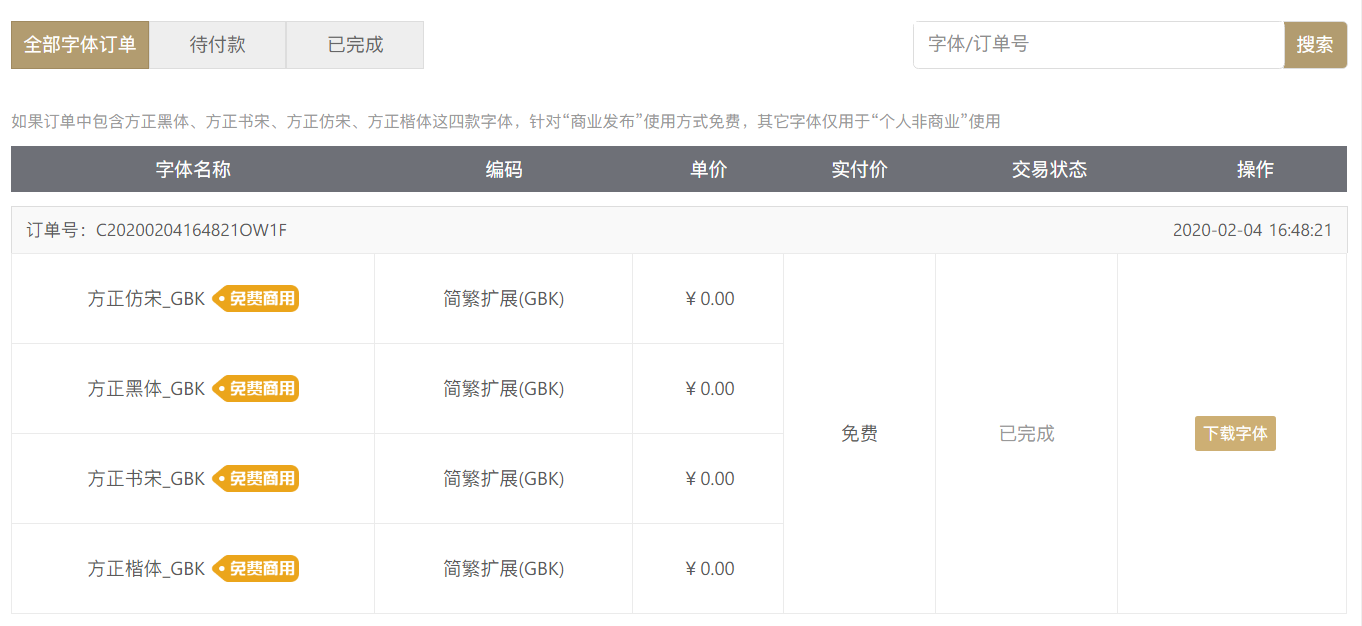
\includegraphics[width=0.9\textwidth]{founder.png}
\end{figure}
\subsection{其他中文字体}
如果你想完全自定义字体\footnote{这里仍然以方正字体为例。},你可以选择 \lstinline{chinesefont=nofont},然后在导言区设置
\begin{lstlisting}
\setCJKmainfont[BoldFont={FZHei-B01},ItalicFont={FZKai-Z03}]{FZShuSong-Z01}
\setCJKsansfont[BoldFont={FZHei-B01}]{FZKai-Z03}
\setCJKmonofont[BoldFont={FZHei-B01}]{FZFangSong-Z02}
\setCJKfamilyfont{zhsong}{FZShuSong-Z01}
\setCJKfamilyfont{zhhei}{FZHei-B01}
\setCJKfamilyfont{zhkai}[BoldFont={FZHei-B01}]{FZKai-Z03}
\setCJKfamilyfont{zhfs}[BoldFont={FZHei-B01}]{FZFangSong-Z02}
\newcommand*{\songti}{\CJKfamily{zhsong}}
\newcommand*{\heiti}{\CJKfamily{zhhei}}
\newcommand*{\kaishu}{\CJKfamily{zhkai}}
\newcommand*{\fangsong}{\CJKfamily{zhfs}}
\end{lstlisting}



\begin{solution}
	即 $D(x)$ 在 $[0,1]$ 上是 Lebesgue 可积的并且积分值为零。但 $D(x)$ 在 $[0,1]$ 上不是 Riemann 可积的。
\end{solution}

\begin{proof}
	即 $D(x)$ 在 $[0,1]$ 上是 Lebesgue 可积的并且积分值为零。但 $D(x)$ 在 $[0,1]$ 上不是 Riemann 可积的。
\end{proof}

\begin{theorem}[Fubini 定理] \label{thm:fubi}
	(1)若 $f(x,y)$ 是 $\mathcal{R}^p\times\mathcal{R}^q$ 上的非负可测函数,则对几乎处处的 $x\in \mathcal{R}^p$,$f(x,y)$ 作为 $y$ 的函数是 $\mathcal{R}^q$ 上的非负可测函数,$g(x)=\int_{\mathcal{R}^q}f(x,y) dy$ 是 $\mathcal{R}^p$ 上的非负可测函数。并且
	\begin{equation}
		\label{eq:461}
		\int_{\mathcal{R}^p\times\mathcal{R}^q} f(x,y) dxdy=\int_{\mathcal{R}^p}\left(\int_{\mathcal{R}^q}f(x,y)dy\right)dx.
	\end{equation}

	(2)若 $f(x,y)$ 是 $\mathcal{R}^p\times\mathcal{R}^q$ 上的可积函数,则对几乎处处的 $x\in\mathcal{R}^p$,$f(x,y)$ 作为 $y$ 的函数是 $\mathcal{R}^q$ 上的可积函数,并且 $g(x)=\int_{\mathcal{R}^q}f(x,y) dy$ 是 $\mathcal{R}^p$ 上的可积函数。而且~\eqref{eq:461} 成立。
\end{theorem}

\begin{note}
	在本模板中,引理(lemma),推论(corollary)的样式和定理~\ref{thm:fubi} 的样式一致,包括颜色,仅仅只有计数器的设置不一样。
\end{note}

我们说一个实变或者复变量的实值或者复值函数是在区间上平方可积的,如果其绝对值的平方在该区间上的积分是有限的。所有在勒贝格积分意义下平方可积的可测函数构成一个希尔伯特空间,也就是所谓的 $L^2$ 空间,几乎处处相等的函数归为同一等价类。形式上,$L^2$ 是平方可积函数的空间和几乎处处为 0 的函数空间的商空间。

\begin{proposition}[最优性原理] \label{pro:max}
	如果 $u^*$ 在 $[s,T]$ 上为最优解,则 $u^*$ 在 $[s, T]$ 任意子区间都是最优解,假设区间为 $[t_0, t_1]$ 的最优解为 $u^*$ ,则 $u(t_0)=u^{*}(t_0)$,即初始条件必须还是在 $u^*$ 上。
\end{proposition}

我们知道最小二乘法可以用来处理一组数据,可以从一组测定的数据中寻求变量之间的依赖关系,这种函数关系称为经验公式。本课题将介绍最小二乘法的精确定义及如何寻求点与点之间近似成线性关系时的经验公式。假定实验测得变量之间的 $n$ 个数据,则在平面上,可以得到 $n$ 个点,这种图形称为 “散点图”,从图中可以粗略看出这些点大致散落在某直线近旁, 我们认为其近似为一线性函数,下面介绍求解步骤。

\begin{figure}[htbp]
	\centering
	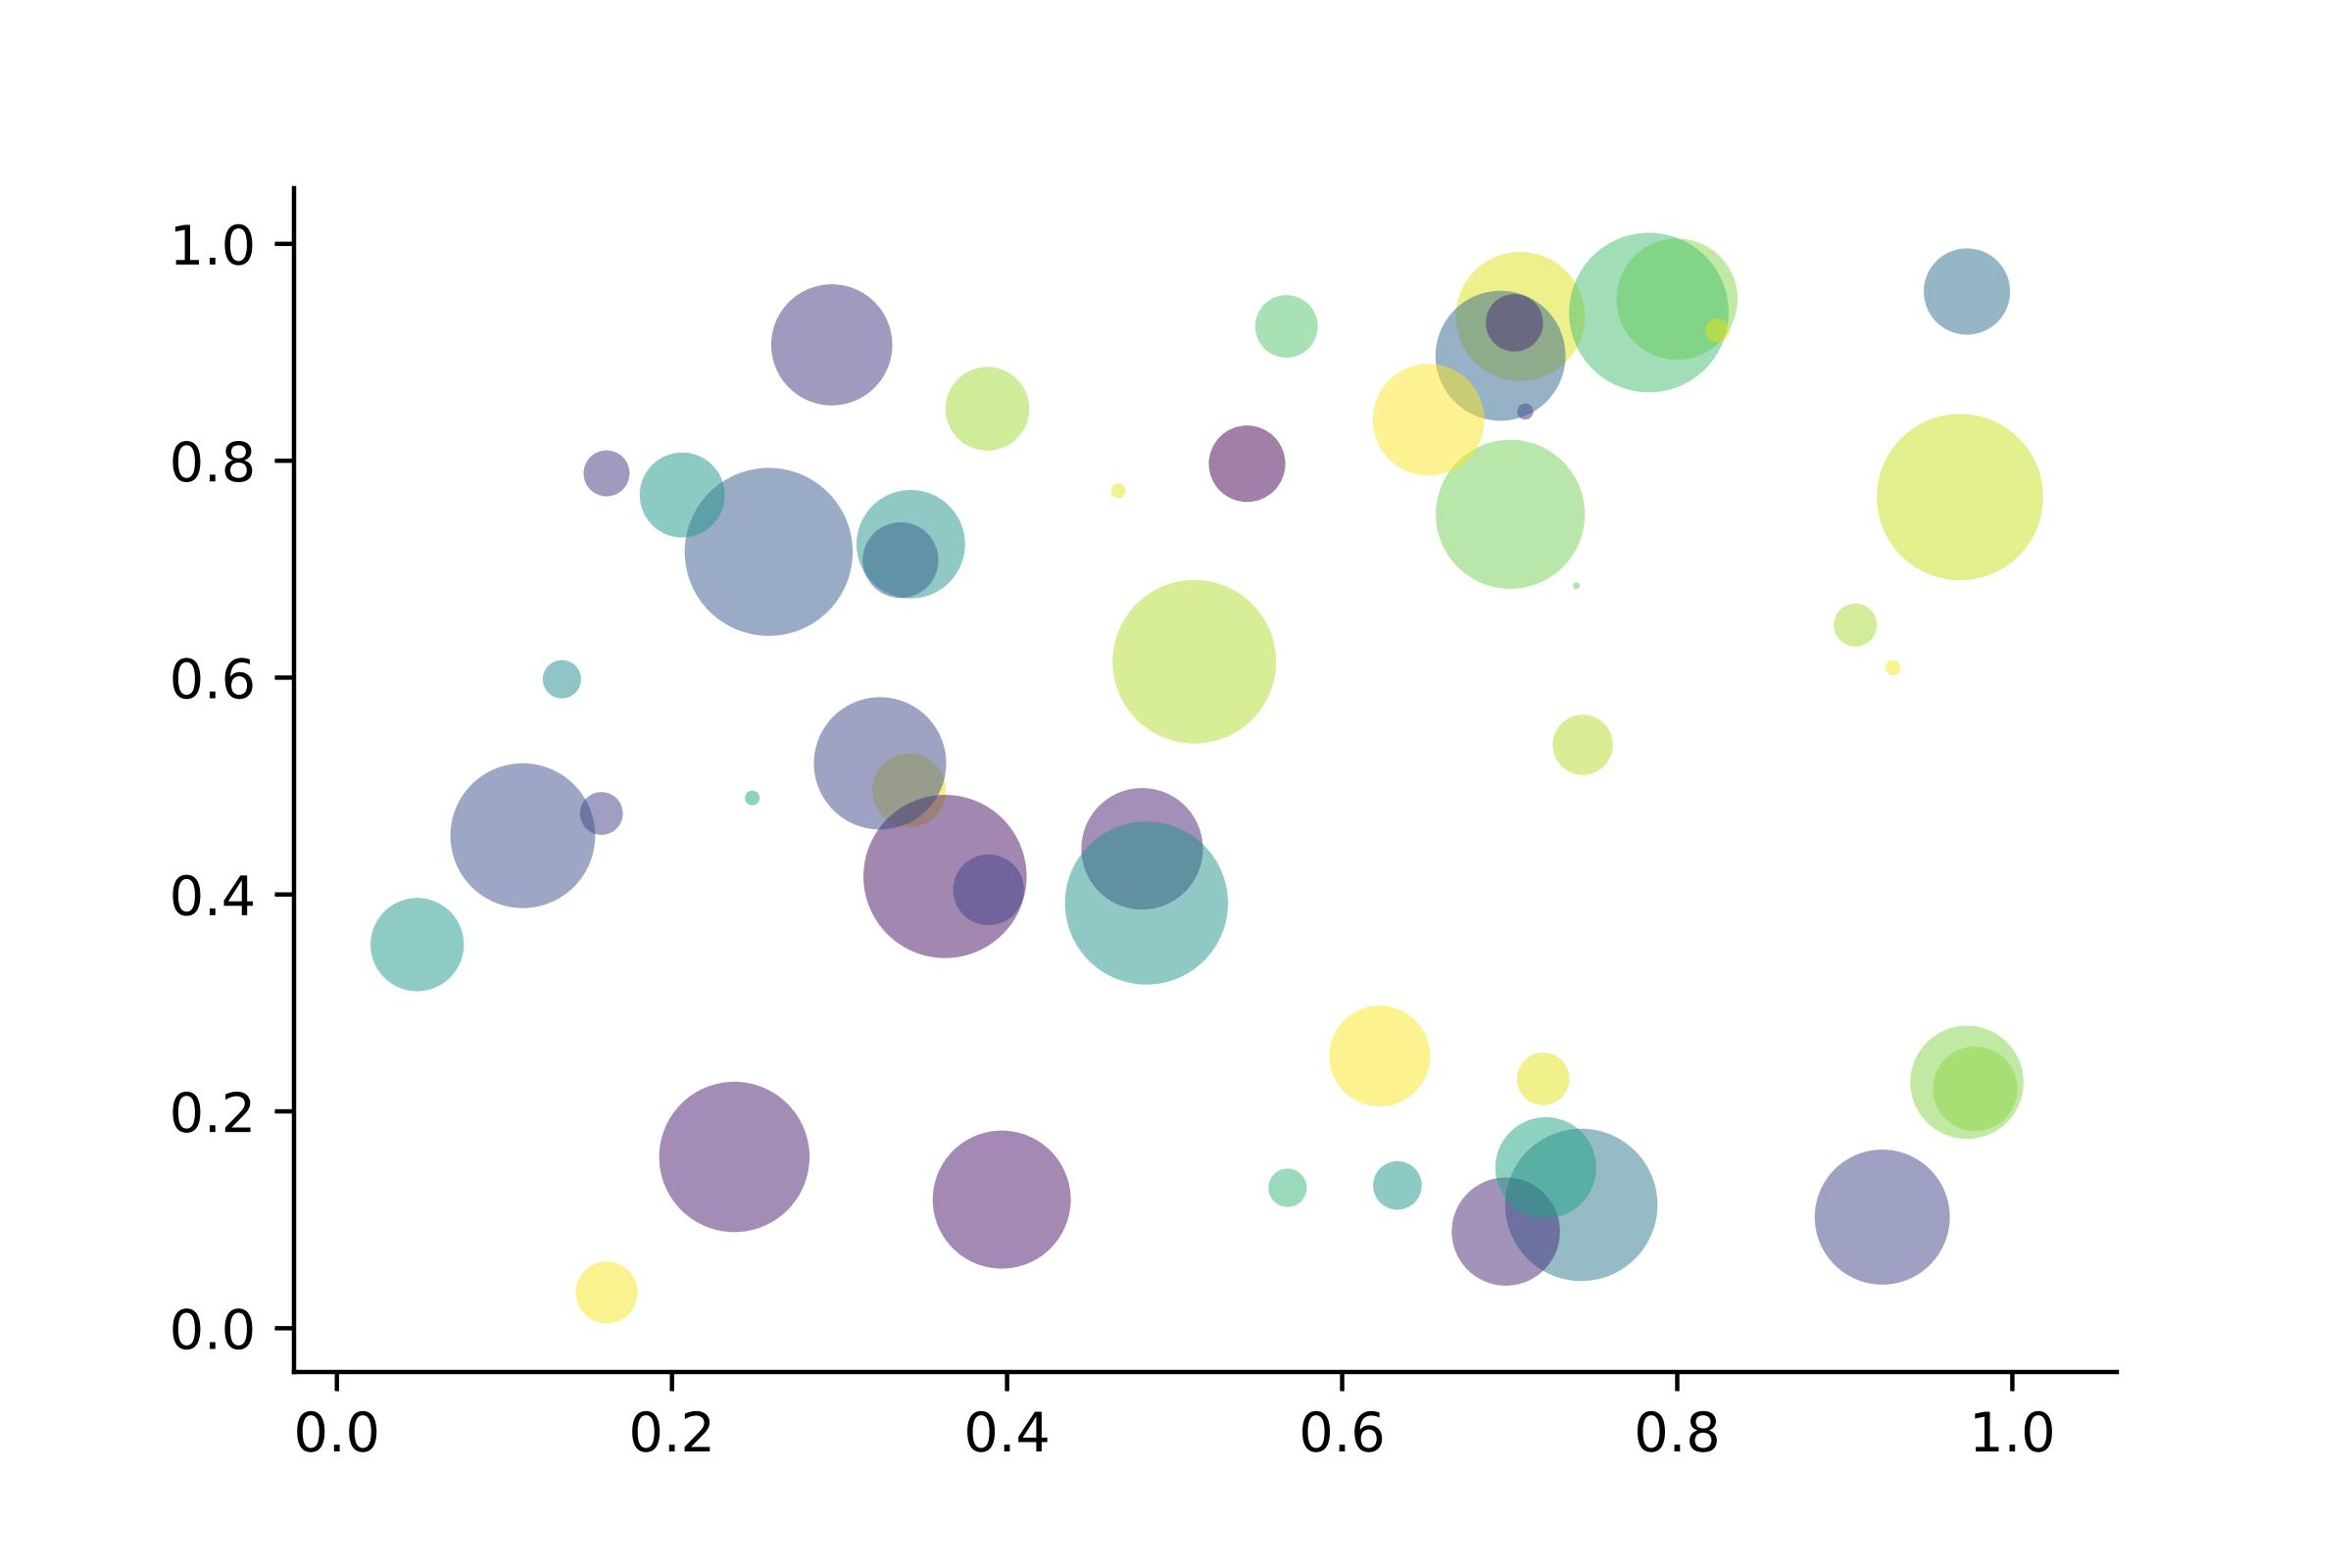
\includegraphics[width=0.6\textwidth]{scatter.jpg}
	\caption{散点图示例 $\hat{y}=a+bx$ \label{fig:scatter}}
\end{figure}

以最简单的一元线性模型来解释最小二乘法。什么是一元线性模型呢?监督学习中,如果预测的变量是离散的,我们称其为分类(如决策树,支持向量机等),如果预测的变量是连续的,我们称其为回归。回归分析中,如果只包括一个自变量和一个因变量,且二者的关系可用一条直线近似表示,这种回归分析称为一元线性回归分析。如果回归分析中包括两个或两个以上的自变量,且因变量和自变量之间是线性关系,则称为多元线性回归分析。对于二维空间线性是一条直线;对于三维空间线性是一个平面,对于多维空间线性是一个超平面。

\begin{property}\label{property:cauchy}
	柯西列的性质
	\begin{enumerate}
		\item $\{x_k\}$ 是柯西列,则其子列 $\{x_k^i\}$ 也是柯西列。
		\item $x_k\in \mathcal{R}^n$,$\rho(x,y)$ 是欧几里得空间,则柯西列收敛,$(\mathcal{R}^n,\rho)$ 空间是完备的。
	\end{enumerate}
\end{property}

\begin{conclusion}
	回归分析(regression analysis) 是确定两种或两种以上变量间相互依赖的定量关系的一种统计分析方法。运用十分广泛,回归分析按照涉及的变量的多少,分为一元回归和多元回归分析;按照因变量的多少,可分为简单回归分析和多重回归分析;按照自变量和因变量之间的关系类型,可分为线性回归分析和非线性回归分析。
\end{conclusion}

\begin{problemset}
	\item 设 $A$ 为数域 $K$ 上的 $n$ 级矩阵。证明:如果 $K^n$ 中任意非零列向量都是 $A$ 的特征向量,则 $A$ 一定是数量矩阵。
	\item 证明:不为零矩阵的幂零矩阵不能对角化。
	\item 设 $A = (a_{ij})$ 是数域 $K$ 上的一个 $n$ 级上三角矩阵,证明:如果 $a_{11} = a_{22} = \cdots = a_{nn}$,并且至少有一个 $a_{kl} \not = 0 (k < l)$,则 $A$ 一定不能对角化。
\end{problemset}

\chapter{常见问题集}

我们根据用户社区反馈整理了下面一些常见的问题,用户在遇到问题时,应当首先查阅本手册和本部分的常见的问题。

\begin{enumerate}[itemsep=1.5ex]
	\item \question{有没有办法章节用“第一章,第一节,(一)”这种?}
	      见前文介绍,可以使用 \lstinline{scheme=chinese} 设置。
	\item \question{大佬,我想把正文字体改为亮色,背景色改为黑灰色。}
	      页面颜色可以使用 \lstinline{\pagecolor} 命令设置,文本命令可以参考\href{https://tex.stackexchange.com/questions/278544/xcolor-what-is-the-equivalent-of-default-text-color}{这里}进行设置。
	\item \question{\lstinline{! LaTeX Error: Unknown option 'scheme=plain' for package 'ctex'.}}
	      你用的 C\TeX{} 套装吧?这个里面的 \lstinline{ctex} 宏包已经是已经是 10 年前的了,与本模板使用的 \lstinline{ctex} 宏集有很大区别。不建议 C\TeX{} 套装了,请卸载并安装 \TeX{} Live 2022。
	\item \question{我该使用什么版本?}
	      请务必使用\href{https://github.com/ElegantLaTeX/ElegantBook/releases}{最新正式发行版},发行版间不定期可能会有更新(修复 bug 或者改进之类),如果你在使用过程中没有遇到问题,不需要每次更新\href{https://github.com/ElegantLaTeX/ElegantBook/archive/master.zip}{最新版},但是在发行版更新之后,请尽可能使用最新版(发行版)!最新发行版可以在 GitHub 或者 \TeX{} Live 2021 内获取。
	\item \question{我该使用什么编辑器?}
	      你可以使用 \TeX{} Live 2021 自带的编辑器 \TeX{}works 或者使用 \TeX{}studio,\TeX works 的自动补全,你可以参考我们的总结 \href{https://github.com/EthanDeng/texworks-autocomplete}{\TeX works 自动补全}。推荐使用 \TeX{} Live 2021 + \TeX{}studio。我自己用 VS Code 和 Sublime Text,相关的配置说明,请参考 \href{https://github.com/EthanDeng/vscode-latex}{\LaTeX{} 编译环境配置:Visual Studio Code 配置简介} 和 \href{https://github.com/EthanDeng/sublime-text-latex}{Sublime Text 搭建 \LaTeX{} 编写环境}。
	\item \question{您好,我们想用您的 ElegantBook 模板写一本书。关于机器学习的教材,希望获得您的授权,谢谢您的宝贵时间。}
	      模板的使用修改都是自由的,你们声明模板来源以及模板地址(GitHub 地址)即可,其他未尽事宜按照开源协议 LPPL-1.3c。做好之后,如果方便的话,可以给我们一个链接,我把你们的教材放在 Elegant\LaTeX{} 用户作品集里。
	\item \question{请问交叉引用是什么?}
	      本群和本模板适合有一定 \LaTeX{} 基础的用户使用,新手请先学习 \LaTeX{} 的基础,理解各种概念,否则你将寸步难行。
	\item \question{代码高亮环境能用其他语言吗?}
	      可以的,ElegantBook 模板用的是 \lstinline{listings} 宏包,你可以在环境(\lstinline{lstlisting})之后加上语言(比如 Python 使用 \lstinline{language=Python} 选项),全局语言修改请使用 \lstinline{lstset} 命令,更多信息请参考宏包文档。
	\item \question{群主,什么时候出 Beamer 的模板(主题),ElegantSlide 或者 ElegantBeamer?}
	      由于 Beamer 中有一个很优秀的主题 \href{https://github.com/matze/mtheme}{Metropolis}。后续确定不会再出任何主题/模板,请大家根据需要修改已有主题。
\end{enumerate}

\chapter{版本更新历史}

根据用户的反馈,我们不断修正和完善模板。由于 3.00 之前版本与现在版本差异非常大,在此不列出 3.00 之前的更新内容。

\datechange{2022/12/31}{版本 4.5} \textcolor{red}{\bfseries 停止维护!}

\datechange{2022/08/17}{版本 4.5 pre}
\begin{change}
	\item \textbf{重要改动}:提供了一个新的文档类选项 \lstinline|usesamecnt|,可以使全局的定理类环境使用同一个计数器。
	\item \textbf{重要改动}:修改了 \lstinline|\elegantnewtheorem| 命令,使其有第五个(可选)参数。
\end{change}

\datechange{2022/08/15}{版本 4.4 正式发布。}

\begin{change}
	\item \textbf{重要改动}:提供了一个定义定理类环境的命令 \lstinline|\elegantnewtheorem|;
	\item \textbf{重要改动}:为所有内置定理类环境提供了带星号的版本,带星号的定理类环境不会编号,修复 \href{https://github.com/ElegantLaTeX/ElegantBook/issues/167}{issue: \#167};
	\item \textbf{重要改动}:在 \lstinline{scheme=chinese} 下将目录中的“第 1 章”修改为“第一章”;
	\item 将 TeX Gyre Termes 改为 TeX Gyre TermesX,使英文部分字形与 newtx 系列宏包更相近;
	\item 重写了内置定理类环境的实现方法,修复了一些 bug,由于修改部分较大,如果引入了新的 bug,请及时在 QQ 群或 \href{https://github.com/ElegantLaTeX}{Github} 上进行反馈;
	\item 删除 Gitee 仓库地址,恢复 GitHub 提交(pull requests);
	\item 将参考文献命令添加到导言区,使编辑器能够对参考文献自动补全。
\end{change}

\datechange{2022/04/09}{版本 4.3 正式发布。}

\begin{change}
	\item 放弃 newtx 系列宏包的设置,改用 TeX Gyre Termes,并设置其他字体;
	\item 修改定理类环境内部字体设置,修复环境内部中文无法加粗问题;
	\item 增加定理类环境的计数器选项 \lstinline{thmcnt},可选 \lstinline{chapter} 和 \lstinline{section};
	\item 增加 \lstinline{bibend} 选项,可选 \lstinline{bibend=biber}(默认)和 \lstinline{bibend=bibtex}。
\end{change}



\datechange{2022/03/08}{版本 4.2 正式发布。}

\begin{change}
	\item 对于 newtx 系列宏包更新导致的字体 bug 的修复;
	\item 修缮目录格式,为了达到这个目的,重新改写 \lstinline{\chaptername} 的重定义语句;
	\item 增加日语 \lstinline{lang=jp} 设定。
	\item 这个版本为一个临时性版本,在 \TeX Live 2022 发布之后,将尽快发布 4.3 版本,由于对于中文的改动比较大,可能会出现预期之外的 bug,有问题可以在 QQ 群或者 Github 反馈。
\end{change}


\datechange{2021/05/02}{版本 4.1 正式发布。}

\begin{change}
	\item \textbf{重要改动}:由原先的 \hologo{BibTeX} 改为 biblatex 编译方式(后端为 \lstinline{biber}),请注意两者之间的差异;
	\item \textbf{重要改进}:修改对于定理写法兼容方式,提高数学公式代码的兼容性;
	\item 页面设置改动,默认页面更宽;方便书写和阅读;
	\item 支持目录文字以及页码跳转;
	\item 不再维护 \hologo{pdfLaTeX} 中文支持方式,请务必使用 \hologo{XeLaTeX} 编译中文文稿。
	\item 增加多个语言选项,法语 \lstinline{lang=fr}、荷兰语 \lstinline{lang=nl}、匈牙利语 \lstinline{lang=hu}、西班牙语 \lstinline{lang=es}、蒙古语 \lstinline{lang=mn} 等。
\end{change}


\datechange{2020/04/12}{版本 3.11 正式发布,\textcolor{red}{此版本为 3.x 最后版本。}}

\begin{change}
	\item \textbf{重要修正}:修复因为 \lstinline{gbt7714} 宏包更新导致的 \lstinline{natbib option clash} 错误;
	\item 由于 \lstinline{pgfornament} 宏包未被 \TeX{} Live 2020 收录,因此删除 base 相关的内容;
	\item 修复部分环境的空格问题;
	\item 增加了意大利语言选项 \lstinline{lang=it}。
\end{change}


\datechange{2020/02/10}{版本 3.10 正式发布}

\begin{change}
	\item 增加数学字体选项 \lstinline{math},可选项为 \lstinline{newtx} 和 \lstinline{cm}。\\
	\textbf{重要提示}:原先通过 \lstinline{newtxmath} 宏包设置的数学字体改为 \LaTeX{} 默认数学字体,如果需要保持原来的字体,需要显式声明数学字体(\lstinline{math=newtx});
	\item 新增中文字体选项 \lstinline{chinesefont},可选项为 \lstinline{ctexfont}、\lstinline{founder} 和 \lstinline{nofont}。
	\item 将封面作者信息设置为可选,并且增加自定义信息命令 \lstinline{\bioinfo};
	\item 在说明文档中增加版本历史,新增 \lstinline{\datechange} 命令和 \lstinline{change} 环境;
	\item 增加汉化章节选项 \lstinline{scheme},可选项为汉化 \lstinline{chinese};
	\item 由于 \lstinline{\lvert} 问题已经修复,重新调整 \lstinline{ctex} 宏包和 \lstinline{amsmath} 宏包位置。
	\item 修改页眉设置,去除了 \lstinline{\lastpage} 以避免 page anchor 问题,加入 \lstinline{\frontmatter}。
	\item 修改参考文献选项 \lstinline{cite},可选项为数字 \lstinline{numbers}、 作者-年份 \lstinline{authoryear} 以及上标 \lstinline{super}。
	\item 新增参考文献样式选项 \lstinline{bibstyle},并将英文模式下参考文献样式 \lstinline{apalike} 设置为默认值,中文仍然使用 \lstinline{gbt7714} 宏包设置。
\end{change}

\datechange{2019/08/18}{版本 3.09 正式发布}

\begin{change}
	\item \lstinline{\elegantpar} 存在 bug,删除 \lstinline{\elegantpar} 命令,建议用户改用 \lstinline{\marginnote} 和 \lstinline{\marginpar} 旁注命令。
	\item 积分操作符统一更改为 \lstinline{esint} 宏包设置;
	\item 新增目录选项 \lstinline{toc},可选项为单栏 \lstinline{onecol} 和双栏 \lstinline{twocol};
	\item 手动增加参考文献选项 \lstinline{cite},可选项为上标形式 \lstinline{super};
	\item 修正章节习题(\lstinline{problemset})环境。
\end{change}

\datechange{2019/05/28}{版本 3.08 正式发布}

\begin{change}
	\item 修复 \lstinline{\part} 命令。
	\item 引入 Note 模板中的 \lstinline{pad} 选项 \lstinline{device=pad}。
	\item 数学字体加入 \lstinline{mtpro2} 可选项 \lstinline{math=mtpro2},使用免费的 \lstinline{lite} 子集。
	\item 将参考文献默认显示方式 \lstinline{authoyear} 改为 \lstinline{numbers}。
	\item 引入旁注命令 \lstinline{\marginpar}(测试)。
	\item 新增章节摘要环境 \lstinline{introduction}。
	\item 新增章节习题环境 \lstinline{problemset}。
	\item 将 \lstinline{\equote} 重命名为 \lstinline{\extrainfo}。
	\item 完善说明文档,增加致谢部分。
\end{change}

\datechange{2019/04/15}{版本 3.07 正式发布}

\begin{change}
	\item 删除中英文自定义字体总设置。
	\item 新增颜色主题,并将原绿色默认主题设置为蓝色 \lstinline{color=blue}。
	\item 引入隐藏装饰图案选项 \lstinline{base},可选项有显示 \lstinline{show} 和隐藏 \lstinline{hide}。
	\item 新增定理模式 \lstinline{mode},可选项有简单模式 \lstinline{simple} 和炫彩模式 \lstinline{fancy}。
	\item 新增隐藏证明、答案等环境的选项 \lstinline{result=noanswer}。
\end{change}

\datechange{2019/02/25}{版本 3.06 正式发布}

\begin{change}
	\item 删除水印。
	\item 新封面,新装饰图案。
	\item 添加引言使用说明。
	\item 修复双面 \lstinline{twoside}。
	\item 美化列表环境。
	\item 增加 \lstinline{\subsubsection} 的设置。
	\item 将模板拆分成中英文语言模式。
	\item 使用 \lstinline{lstlisting} 添加代码高亮。
	\item 增加定理类环境使用说明。
\end{change}

\datechange{2019/01/22}{版本 3.05 正式发布}

\begin{change}
	\item 添加 \lstinline{xeCJK} 宏包中文支持方案。
	\item 修复模板之前对 Ti\textit{k}Z 单位的改动。
	\item 更新 logo 图。
\end{change}

\datechange{2019/01/15}{版本 3.04 正式发布}

\begin{change}
	\item 格式化模板代码。
	\item 增加 \lstinline{\equote} 命令。
	\item 修改 \lstinline{\date}。
\end{change}

\datechange{2019/01/08}{版本 3.03 正式发布}

\begin{change}
	\item 修复附录章节显示问题。
	\item 小幅优化封面代码。
\end{change}

\datechange{2018/12/31}{版本 3.02 正式发布}

\begin{change}
	\item 修复名字系列命令自定义格式时出现的空格问题,比如 \lstinline{\listfigurename}。
	\item 英文定理类名字改为中文名。
	\item 英文结构名改为中文。
\end{change}

\datechange{2018/12/16}{版本 3.01 正式发布}

\begin{change}
	\item 调整 \lstinline{ctex} 宏包。
	\item 说明文档增加更新内容。
\end{change}

\datechange{2018/12/06}{版本 3.00 正式发布}

\begin{change}
	\item 删除 \lstinline{mathpazo} 数学字体选项。
	\item 添加邮箱命令 \lstinline{\mailto}。
	\item 修改英文字体为 \lstinline{newtx} 系列,另外大型操作符号维持 cm 字体。
	\item 中文字体改用 \lstinline{ctex} 宏包自动设置。
	\item 删除 \lstinline{xeCJK} 字体设置,原因是不同系统字体不方便统一。
	\item 定理换用 \lstinline{tcolorbox} 宏包定义,并基本维持原有的定理样式,优化显示效果,支持跨页;定理类名字重命名,如 etheorem 改为 theorem 等等。
	\item 删去自定义的缩进命令 \lstinline{\Eindent}。
	\item 添加参考文献宏包 \lstinline{natbib}。
	\item 颜色名字重命名。
\end{change}

\nocite{*}

\printbibliography[heading=bibintoc, title=\ebibname]
\appendix


\section{23真题考场做题思路}
\begin{exercise}在中方支持下,2023 年 3 月 6 日至 10 日,沙特阿拉伯与伊朗在北京举行对话。3 月 10日,中沙伊三方签署并发表联合声明,宜布沙伊双方同意恢复外交关系。这是党的二十大后 中国外交的“大手笔”。中方推动沙伊握手言和的重要意义表现在
	\begin{choice}
		\item 创造了调解冲突的新范式,为其他地区热点问题的解决提供了新思路
		\item 使沙伊矛盾得以最终解决
		\item 助力中东地区实现和平、稳定与安全
		\item 为国际社会注入和平合作的正能量
	\end{choice}
\end{exercise}
\section{22真题考场做题思路}
\section{21真题考场做题思路}
\section{20真题考场做题思路}
\section{19真题考场做题思路}
\section{18真题考场做题思路}
\section{17真题考场做题思路}
\section{16真题考场做题思路}
\section{15真题考场做题思路}
\section{14真题考场做题思路}
\section{13真题考场做题思路}
\section{12真题考场做题思路}
\section{11真题考场做题思路}
\section{10真题考场做题思路}

\chapter{浅谈主观题得高分要素}





\chapter{主观题利器——答题逻辑}

\section{官方参考答案分析}



\section{答题逻辑}

\subsection{马原答题逻辑}
\subsection{新思想答题逻辑}
\subsection{史纲答题逻辑}
\subsection{毛中特答题逻辑}
\subsection{思修答题逻辑}
\subsection{时政答题逻辑}

\chapter{杂谈}
\section{如何背肖四}
\section{最后一个月该如何高效备考}

\end{document}

